\documentclass[11pt]{article}
\renewcommand{\arraystretch}{1.5} % Default value: 1
\usepackage{sectsty}
\allsectionsfont{\color{blue}\fontfamily{lmss}\selectfont}
\usepackage{fontspec}
\setmainfont{XCharter}

\usepackage{listings}
\lstset{
basicstyle=\small\ttfamily,
tabsize=8,
columns=flexible,
breaklines=true,
frame=tb,
rulecolor=\color[rgb]{0.8,0.8,0.7},
backgroundcolor=\color[rgb]{1,1,0.91},
postbreak=\raisebox{0ex}[0ex][0ex]{\ensuremath{\color{red}\hookrightarrow\space}}
}
\usepackage{fontawesome}


\usepackage{mdframed}
\newmdenv[
  backgroundcolor=gray,
  fontcolor=white,
  nobreak=true,
]{terminalinput}



\usepackage{parskip}




    \usepackage[T1]{fontenc}
    % Nicer default font than Computer Modern for most use cases
    \usepackage{palatino}

    % Basic figure setup, for now with no caption control since it's done
    % automatically by Pandoc (which extracts ![](path) syntax from Markdown).
    \usepackage{graphicx}
    % We will generate all images so they have a width \maxwidth. This means
    % that they will get their normal width if they fit onto the page, but
    % are scaled down if they would overflow the margins.
    \makeatletter
    \def\maxwidth{\ifdim\Gin@nat@width>\linewidth\linewidth
    \else\Gin@nat@width\fi}
    \makeatother
    \let\Oldincludegraphics\includegraphics
    % Set max figure width to be 80% of text width, for now hardcoded.
\renewcommand{\includegraphics}[1]{\Oldincludegraphics[width=.8\maxwidth, height=.55\textheight, keepaspectratio]{#1}}
    % Ensure that by default, figures have no caption (until we provide a
    % proper Figure object with a Caption API and a way to capture that
    % in the conversion process - todo).
    \usepackage{caption}
    \DeclareCaptionLabelFormat{nolabel}{}
    \captionsetup{labelformat=nolabel, textfont=bf}

    \usepackage{adjustbox} % Used to constrain images to a maximum size
    \usepackage{xcolor} % Allow colors to be defined
    \usepackage{enumerate} % Needed for markdown enumerations to work
    \usepackage{geometry} % Used to adjust the document margins
    \usepackage{amsmath} % Equations
    \usepackage{amssymb} % Equations
    \usepackage{textcomp} % defines textquotesingle
    % Hack from http://tex.stackexchange.com/a/47451/13684:
    \AtBeginDocument{%
        \def\PYZsq{\textquotesingle}% Upright quotes in Pygmentized code
    }
    \usepackage{upquote} % Upright quotes for verbatim code
    \usepackage{eurosym} % defines \euro
    \usepackage[mathletters]{ucs} % Extended unicode (utf-8) support
    \usepackage[utf8x]{inputenc} % Allow utf-8 characters in the tex document
    \usepackage{fancyvrb} % verbatim replacement that allows latex
    \usepackage{grffile} % extends the file name processing of package graphics
                         % to support a larger range
    % The hyperref package gives us a pdf with properly built
    % internal navigation ('pdf bookmarks' for the table of contents,
    % internal cross-reference links, web links for URLs, etc.)
    \usepackage{hyperref}
    \usepackage{longtable} % longtable support required by pandoc >1.10
    \usepackage{booktabs}  % table support for pandoc > 1.12.2
    \usepackage[normalem]{ulem} % ulem is needed to support strikethroughs (\sout)
                                % normalem makes italics be italics, not underlines
    \usepackage{float}



    % Colors for the hyperref package
    \definecolor{urlcolor}{rgb}{0,.145,.698}
    \definecolor{linkcolor}{rgb}{.71,0.21,0.01}
    \definecolor{citecolor}{rgb}{.12,.54,.11}

    % ANSI colors
    \definecolor{ansi-black}{HTML}{3E424D}
    \definecolor{ansi-black-intense}{HTML}{282C36}
    \definecolor{ansi-red}{HTML}{E75C58}
    \definecolor{ansi-red-intense}{HTML}{B22B31}
    \definecolor{ansi-green}{HTML}{00A250}
    \definecolor{ansi-green-intense}{HTML}{007427}
    \definecolor{ansi-yellow}{HTML}{DDB62B}
    \definecolor{ansi-yellow-intense}{HTML}{B27D12}
    \definecolor{ansi-blue}{HTML}{208FFB}
    \definecolor{ansi-blue-intense}{HTML}{0065CA}
    \definecolor{ansi-magenta}{HTML}{D160C4}
    \definecolor{ansi-magenta-intense}{HTML}{A03196}
    \definecolor{ansi-cyan}{HTML}{60C6C8}
    \definecolor{ansi-cyan-intense}{HTML}{258F8F}
    \definecolor{ansi-white}{HTML}{C5C1B4}
    \definecolor{ansi-white-intense}{HTML}{A1A6B2}

    % commands and environments needed by pandoc snippets
    % extracted from the output of `pandoc -s`
    \providecommand{\tightlist}{%
      \setlength{\itemsep}{0pt}\setlength{\parskip}{0pt}}
    \DefineVerbatimEnvironment{Highlighting}{Verbatim}{commandchars=\\\{\}}
    % Add ',fontsize=\small' for more characters per line
    \newenvironment{Shaded}{}{}
    \newcommand{\KeywordTok}[1]{\textcolor[rgb]{0.00,0.44,0.13}{\textbf{{#1}}}}
    \newcommand{\DataTypeTok}[1]{\textcolor[rgb]{0.56,0.13,0.00}{{#1}}}
    \newcommand{\DecValTok}[1]{\textcolor[rgb]{0.25,0.63,0.44}{{#1}}}
    \newcommand{\BaseNTok}[1]{\textcolor[rgb]{0.25,0.63,0.44}{{#1}}}
    \newcommand{\FloatTok}[1]{\textcolor[rgb]{0.25,0.63,0.44}{{#1}}}
    \newcommand{\CharTok}[1]{\textcolor[rgb]{0.25,0.44,0.63}{{#1}}}
    \newcommand{\StringTok}[1]{\textcolor[rgb]{0.25,0.44,0.63}{{#1}}}
    \newcommand{\CommentTok}[1]{\textcolor[rgb]{0.38,0.63,0.69}{\textit{{#1}}}}
    \newcommand{\OtherTok}[1]{\textcolor[rgb]{0.00,0.44,0.13}{{#1}}}
    \newcommand{\AlertTok}[1]{\textcolor[rgb]{1.00,0.00,0.00}{\textbf{{#1}}}}
    \newcommand{\FunctionTok}[1]{\textcolor[rgb]{0.02,0.16,0.49}{{#1}}}
    \newcommand{\RegionMarkerTok}[1]{{#1}}
    \newcommand{\ErrorTok}[1]{\textcolor[rgb]{1.00,0.00,0.00}{\textbf{{#1}}}}
    \newcommand{\NormalTok}[1]{{#1}}

    % Additional commands for more recent versions of Pandoc
    \newcommand{\ConstantTok}[1]{\textcolor[rgb]{0.53,0.00,0.00}{{#1}}}
    \newcommand{\SpecialCharTok}[1]{\textcolor[rgb]{0.25,0.44,0.63}{{#1}}}
    \newcommand{\VerbatimStringTok}[1]{\textcolor[rgb]{0.25,0.44,0.63}{{#1}}}
    \newcommand{\SpecialStringTok}[1]{\textcolor[rgb]{0.73,0.40,0.53}{{#1}}}
    \newcommand{\ImportTok}[1]{{#1}}
    \newcommand{\DocumentationTok}[1]{\textcolor[rgb]{0.73,0.13,0.13}{\textit{{#1}}}}
    \newcommand{\AnnotationTok}[1]{\textcolor[rgb]{0.38,0.63,0.69}{\textbf{\textit{{#1}}}}}
    \newcommand{\CommentVarTok}[1]{\textcolor[rgb]{0.38,0.63,0.69}{\textbf{\textit{{#1}}}}}
    \newcommand{\VariableTok}[1]{\textcolor[rgb]{0.10,0.09,0.49}{{#1}}}
    \newcommand{\ControlFlowTok}[1]{\textcolor[rgb]{0.00,0.44,0.13}{\textbf{{#1}}}}
    \newcommand{\OperatorTok}[1]{\textcolor[rgb]{0.40,0.40,0.40}{{#1}}}
    \newcommand{\BuiltInTok}[1]{{#1}}
    \newcommand{\ExtensionTok}[1]{{#1}}
    \newcommand{\PreprocessorTok}[1]{\textcolor[rgb]{0.74,0.48,0.00}{{#1}}}
    \newcommand{\AttributeTok}[1]{\textcolor[rgb]{0.49,0.56,0.16}{{#1}}}
    \newcommand{\InformationTok}[1]{\textcolor[rgb]{0.38,0.63,0.69}{\textbf{\textit{{#1}}}}}
    \newcommand{\WarningTok}[1]{\textcolor[rgb]{0.38,0.63,0.69}{\textbf{\textit{{#1}}}}}


    % Define a nice break command that doesn't care if a line doesn't already
    % exist.
    \def\br{\hspace*{\fill} \\* }
    % Math Jax compatability definitions
    \def\gt{>}
    \def\lt{<}
    % Document parameters
    \title{index}




    % Pygments definitions

\makeatletter
\def\PY@reset{\let\PY@it=\relax \let\PY@bf=\relax%
    \let\PY@ul=\relax \let\PY@tc=\relax%
    \let\PY@bc=\relax \let\PY@ff=\relax}
\def\PY@tok#1{\csname PY@tok@#1\endcsname}
\def\PY@toks#1+{\ifx\relax#1\empty\else%
    \PY@tok{#1}\expandafter\PY@toks\fi}
\def\PY@do#1{\PY@bc{\PY@tc{\PY@ul{%
    \PY@it{\PY@bf{\PY@ff{#1}}}}}}}
\def\PY#1#2{\PY@reset\PY@toks#1+\relax+\PY@do{#2}}

\expandafter\def\csname PY@tok@w\endcsname{\def\PY@tc##1{\textcolor[rgb]{0.73,0.73,0.73}{##1}}}
\expandafter\def\csname PY@tok@c\endcsname{\let\PY@it=\textit\def\PY@tc##1{\textcolor[rgb]{0.25,0.50,0.50}{##1}}}
\expandafter\def\csname PY@tok@cp\endcsname{\def\PY@tc##1{\textcolor[rgb]{0.74,0.48,0.00}{##1}}}
\expandafter\def\csname PY@tok@k\endcsname{\let\PY@bf=\textbf\def\PY@tc##1{\textcolor[rgb]{0.00,0.50,0.00}{##1}}}
\expandafter\def\csname PY@tok@kp\endcsname{\def\PY@tc##1{\textcolor[rgb]{0.00,0.50,0.00}{##1}}}
\expandafter\def\csname PY@tok@kt\endcsname{\def\PY@tc##1{\textcolor[rgb]{0.69,0.00,0.25}{##1}}}
\expandafter\def\csname PY@tok@o\endcsname{\def\PY@tc##1{\textcolor[rgb]{0.40,0.40,0.40}{##1}}}
\expandafter\def\csname PY@tok@ow\endcsname{\let\PY@bf=\textbf\def\PY@tc##1{\textcolor[rgb]{0.67,0.13,1.00}{##1}}}
\expandafter\def\csname PY@tok@nb\endcsname{\def\PY@tc##1{\textcolor[rgb]{0.00,0.50,0.00}{##1}}}
\expandafter\def\csname PY@tok@nf\endcsname{\def\PY@tc##1{\textcolor[rgb]{0.00,0.00,1.00}{##1}}}
\expandafter\def\csname PY@tok@nc\endcsname{\let\PY@bf=\textbf\def\PY@tc##1{\textcolor[rgb]{0.00,0.00,1.00}{##1}}}
\expandafter\def\csname PY@tok@nn\endcsname{\let\PY@bf=\textbf\def\PY@tc##1{\textcolor[rgb]{0.00,0.00,1.00}{##1}}}
\expandafter\def\csname PY@tok@ne\endcsname{\let\PY@bf=\textbf\def\PY@tc##1{\textcolor[rgb]{0.82,0.25,0.23}{##1}}}
\expandafter\def\csname PY@tok@nv\endcsname{\def\PY@tc##1{\textcolor[rgb]{0.10,0.09,0.49}{##1}}}
\expandafter\def\csname PY@tok@no\endcsname{\def\PY@tc##1{\textcolor[rgb]{0.53,0.00,0.00}{##1}}}
\expandafter\def\csname PY@tok@nl\endcsname{\def\PY@tc##1{\textcolor[rgb]{0.63,0.63,0.00}{##1}}}
\expandafter\def\csname PY@tok@ni\endcsname{\let\PY@bf=\textbf\def\PY@tc##1{\textcolor[rgb]{0.60,0.60,0.60}{##1}}}
\expandafter\def\csname PY@tok@na\endcsname{\def\PY@tc##1{\textcolor[rgb]{0.49,0.56,0.16}{##1}}}
\expandafter\def\csname PY@tok@nt\endcsname{\let\PY@bf=\textbf\def\PY@tc##1{\textcolor[rgb]{0.00,0.50,0.00}{##1}}}
\expandafter\def\csname PY@tok@nd\endcsname{\def\PY@tc##1{\textcolor[rgb]{0.67,0.13,1.00}{##1}}}
\expandafter\def\csname PY@tok@s\endcsname{\def\PY@tc##1{\textcolor[rgb]{0.73,0.13,0.13}{##1}}}
\expandafter\def\csname PY@tok@sd\endcsname{\let\PY@it=\textit\def\PY@tc##1{\textcolor[rgb]{0.73,0.13,0.13}{##1}}}
\expandafter\def\csname PY@tok@si\endcsname{\let\PY@bf=\textbf\def\PY@tc##1{\textcolor[rgb]{0.73,0.40,0.53}{##1}}}
\expandafter\def\csname PY@tok@se\endcsname{\let\PY@bf=\textbf\def\PY@tc##1{\textcolor[rgb]{0.73,0.40,0.13}{##1}}}
\expandafter\def\csname PY@tok@sr\endcsname{\def\PY@tc##1{\textcolor[rgb]{0.73,0.40,0.53}{##1}}}
\expandafter\def\csname PY@tok@ss\endcsname{\def\PY@tc##1{\textcolor[rgb]{0.10,0.09,0.49}{##1}}}
\expandafter\def\csname PY@tok@sx\endcsname{\def\PY@tc##1{\textcolor[rgb]{0.00,0.50,0.00}{##1}}}
\expandafter\def\csname PY@tok@m\endcsname{\def\PY@tc##1{\textcolor[rgb]{0.40,0.40,0.40}{##1}}}
\expandafter\def\csname PY@tok@gh\endcsname{\let\PY@bf=\textbf\def\PY@tc##1{\textcolor[rgb]{0.00,0.00,0.50}{##1}}}
\expandafter\def\csname PY@tok@gu\endcsname{\let\PY@bf=\textbf\def\PY@tc##1{\textcolor[rgb]{0.50,0.00,0.50}{##1}}}
\expandafter\def\csname PY@tok@gd\endcsname{\def\PY@tc##1{\textcolor[rgb]{0.63,0.00,0.00}{##1}}}
\expandafter\def\csname PY@tok@gi\endcsname{\def\PY@tc##1{\textcolor[rgb]{0.00,0.63,0.00}{##1}}}
\expandafter\def\csname PY@tok@gr\endcsname{\def\PY@tc##1{\textcolor[rgb]{1.00,0.00,0.00}{##1}}}
\expandafter\def\csname PY@tok@ge\endcsname{\let\PY@it=\textit}
\expandafter\def\csname PY@tok@gs\endcsname{\let\PY@bf=\textbf}
\expandafter\def\csname PY@tok@gp\endcsname{\let\PY@bf=\textbf\def\PY@tc##1{\textcolor[rgb]{0.00,0.00,0.50}{##1}}}
\expandafter\def\csname PY@tok@go\endcsname{\def\PY@tc##1{\textcolor[rgb]{0.53,0.53,0.53}{##1}}}
\expandafter\def\csname PY@tok@gt\endcsname{\def\PY@tc##1{\textcolor[rgb]{0.00,0.27,0.87}{##1}}}
\expandafter\def\csname PY@tok@err\endcsname{\def\PY@bc##1{\setlength{\fboxsep}{0pt}\fcolorbox[rgb]{1.00,0.00,0.00}{1,1,1}{\strut ##1}}}
\expandafter\def\csname PY@tok@kc\endcsname{\let\PY@bf=\textbf\def\PY@tc##1{\textcolor[rgb]{0.00,0.50,0.00}{##1}}}
\expandafter\def\csname PY@tok@kd\endcsname{\let\PY@bf=\textbf\def\PY@tc##1{\textcolor[rgb]{0.00,0.50,0.00}{##1}}}
\expandafter\def\csname PY@tok@kn\endcsname{\let\PY@bf=\textbf\def\PY@tc##1{\textcolor[rgb]{0.00,0.50,0.00}{##1}}}
\expandafter\def\csname PY@tok@kr\endcsname{\let\PY@bf=\textbf\def\PY@tc##1{\textcolor[rgb]{0.00,0.50,0.00}{##1}}}
\expandafter\def\csname PY@tok@bp\endcsname{\def\PY@tc##1{\textcolor[rgb]{0.00,0.50,0.00}{##1}}}
\expandafter\def\csname PY@tok@vc\endcsname{\def\PY@tc##1{\textcolor[rgb]{0.10,0.09,0.49}{##1}}}
\expandafter\def\csname PY@tok@vg\endcsname{\def\PY@tc##1{\textcolor[rgb]{0.10,0.09,0.49}{##1}}}
\expandafter\def\csname PY@tok@vi\endcsname{\def\PY@tc##1{\textcolor[rgb]{0.10,0.09,0.49}{##1}}}
\expandafter\def\csname PY@tok@sb\endcsname{\def\PY@tc##1{\textcolor[rgb]{0.73,0.13,0.13}{##1}}}
\expandafter\def\csname PY@tok@sc\endcsname{\def\PY@tc##1{\textcolor[rgb]{0.73,0.13,0.13}{##1}}}
\expandafter\def\csname PY@tok@s2\endcsname{\def\PY@tc##1{\textcolor[rgb]{0.73,0.13,0.13}{##1}}}
\expandafter\def\csname PY@tok@sh\endcsname{\def\PY@tc##1{\textcolor[rgb]{0.73,0.13,0.13}{##1}}}
\expandafter\def\csname PY@tok@s1\endcsname{\def\PY@tc##1{\textcolor[rgb]{0.73,0.13,0.13}{##1}}}
\expandafter\def\csname PY@tok@mb\endcsname{\def\PY@tc##1{\textcolor[rgb]{0.40,0.40,0.40}{##1}}}
\expandafter\def\csname PY@tok@mf\endcsname{\def\PY@tc##1{\textcolor[rgb]{0.40,0.40,0.40}{##1}}}
\expandafter\def\csname PY@tok@mh\endcsname{\def\PY@tc##1{\textcolor[rgb]{0.40,0.40,0.40}{##1}}}
\expandafter\def\csname PY@tok@mi\endcsname{\def\PY@tc##1{\textcolor[rgb]{0.40,0.40,0.40}{##1}}}
\expandafter\def\csname PY@tok@il\endcsname{\def\PY@tc##1{\textcolor[rgb]{0.40,0.40,0.40}{##1}}}
\expandafter\def\csname PY@tok@mo\endcsname{\def\PY@tc##1{\textcolor[rgb]{0.40,0.40,0.40}{##1}}}
\expandafter\def\csname PY@tok@ch\endcsname{\let\PY@it=\textit\def\PY@tc##1{\textcolor[rgb]{0.25,0.50,0.50}{##1}}}
\expandafter\def\csname PY@tok@cm\endcsname{\let\PY@it=\textit\def\PY@tc##1{\textcolor[rgb]{0.25,0.50,0.50}{##1}}}
\expandafter\def\csname PY@tok@cpf\endcsname{\let\PY@it=\textit\def\PY@tc##1{\textcolor[rgb]{0.25,0.50,0.50}{##1}}}
\expandafter\def\csname PY@tok@c1\endcsname{\let\PY@it=\textit\def\PY@tc##1{\textcolor[rgb]{0.25,0.50,0.50}{##1}}}
\expandafter\def\csname PY@tok@cs\endcsname{\let\PY@it=\textit\def\PY@tc##1{\textcolor[rgb]{0.25,0.50,0.50}{##1}}}

\def\PYZbs{\char`\\}
\def\PYZus{\char`\_}
\def\PYZob{\char`\{}
\def\PYZcb{\char`\}}
\def\PYZca{\char`\^}
\def\PYZam{\char`\&}
\def\PYZlt{\char`\<}
\def\PYZgt{\char`\>}
\def\PYZsh{\char`\#}
\def\PYZpc{\char`\%}
\def\PYZdl{\char`\$}
\def\PYZhy{\char`\-}
\def\PYZsq{\char`\'}
\def\PYZdq{\char`\"}
\def\PYZti{\char`\~}
% for compatibility with earlier versions
\def\PYZat{@}
\def\PYZlb{[}
\def\PYZrb{]}
\makeatother


    % Exact colors from NB
    \definecolor{incolor}{rgb}{0.0, 0.0, 0.5}
    \definecolor{outcolor}{rgb}{0.545, 0.0, 0.0}




    % Prevent overflowing lines due to hard-to-break entities
    \sloppy
    % Setup hyperref package
    \hypersetup{
      breaklinks=true,  % so long urls are correctly broken across lines
      colorlinks=true,
      urlcolor=urlcolor,
      linkcolor=linkcolor,
      citecolor=citecolor,
      }
    % Slightly bigger margins than the latex defaults

    \geometry{verbose,tmargin=1in,bmargin=1in,lmargin=1in,rmargin=1in}



\renewcommand{\PY}[2]{{#2}}
\usepackage{fancyhdr}
\pagestyle{fancy}
\rhead{\color{gray}\sf\small\rightmark}
\lhead{\nouppercase{\color{gray}\sf\small\leftmark}}
\cfoot{\color{gray}\sf\thepage}
\renewcommand{\footrulewidth}{1pt}
\begin{document}






    \hypertarget{deago}{%
\section{DEAGO}\label{deago}}

\hypertarget{introduction}{%
\subsection{Introduction}\label{introduction}}

DEAGO generates user-friendly quality control (QC) and analysis reports
for RNA-Seq datasets. These interactive reports can be opened simply in
a web browser and provide a simple way of sharing information about your
analysis with collaborators.

DEAGO uses a Perl wrapper module
(\textbf{\href{https://github.com/sanger-pathogens/Bio-Deago}{Bio-Deago}})
to generate a HTML report from markdown templates by calling functions
from an R package
(\textbf{\href{https://github.com/sanger-pathogens/deago}{deago}}).

There are three main steps to each analysis:

\begin{itemize}
\tightlist
\item
  Generating QC plots (\textbf{\href{http://ggplot2.org/}{ggplot2}})
\item
  Identifying differentially expressed (DE) genes
  (\textbf{\href{https://bioconductor.org/packages/release/bioc/html/DESeq2.html}{DESeq2}})
\item
  Performing gene ontology (GO) term enrichment analyses
  (\textbf{\href{http://bioconductor.org/packages/release/bioc/html/topGO.html}{topGO}})
\end{itemize}

For more information, please see the
\href{https://github.com/sanger-pathogens/Bio-Deago/blob/master/user_guide/index.ipynb}{user
guide}.

\hypertarget{learning-outcomes}{%
\subsection{Learning outcomes}\label{learning-outcomes}}

By the end of this tutorial you can expect to be able to:

\begin{itemize}
\tightlist
\item
  Understand what input files are required for DEAGO and their formats
\item
  Generate a QC report for an RNA-seq dataset
\item
  Generate a DE report that can be used to identify differentially
  expressed genes
\item
  Generate a GO term enrichment analysis report
\end{itemize}

\hypertarget{tutorial-sections}{%
\subsection{Tutorial sections}\label{tutorial-sections}}

This tutorial comprises the following sections:

\begin{enumerate}
\def\labelenumi{\arabic{enumi}.}
\tightlist
\item
  \href{introduction.ipynb}{Introducing the tutorial dataset}
\item
  \href{input-data.ipynb}{Preparing your input data}
\item
  \href{quality-control.ipynb}{Running a quality control (QC) analysis}
\item
  \href{differential-expression.ipynb}{Running a differential expression
  (DE) analysis}
\item
  \href{go-term-enrichment.ipynb}{Running a GO term enrichment analysis}
\item
  \href{troubleshooting.ipynb}{Troubleshooting}
\end{enumerate}

\hypertarget{authors}{%
\subsection{Authors}\label{authors}}

This tutorial was created by \href{https://github.com/vaofford}{Victoria
Offord}.

\hypertarget{running-the-commands-from-this-tutorial}{%
\subsection{Running the commands from this
tutorial}\label{running-the-commands-from-this-tutorial}}

You can run the commands in this tutorial either directly from the
Jupyter notebook (if using Jupyter), or by typing the commands in your
terminal window.

\hypertarget{running-commands-on-jupyter}{%
\subsubsection{Running commands on
Jupyter}\label{running-commands-on-jupyter}}

If you are using Jupyter, command cells (like the one below) can be run
by selecting the cell and clicking \textit{Cell -\textgreater{} Run} from
the menu above or using \textit{ctrl Enter} to run the command. Let's give
this a try by printing our working directory using the \textit{pwd}
command and listing the files within it. Run the commands in the two
cells below.

\begin{terminalinput}
\begin{Verbatim}[commandchars=\\\{\}]
\llap{\color{black}\LARGE\faKeyboardO\hspace{1em}} \PY{n+nb}{pwd}
\end{Verbatim}
\end{terminalinput}

\begin{terminalinput}
\begin{Verbatim}[commandchars=\\\{\}]
\llap{\color{black}\LARGE\faKeyboardO\hspace{1em}} ls \PYZhy{}l
\end{Verbatim}
\end{terminalinput}

    \hypertarget{running-commands-in-the-terminal}{%
\subsubsection{Running commands in the
terminal}\label{running-commands-in-the-terminal}}

You can also follow this course by typing all the commands you see into
a terminal window. This is similar to the ``Command Prompt'' window on
MS Windows systems, which allows the user to type DOS commands to manage
files.

To get started, select the cell below with the mouse and then either
press control and enter or choose Cell -\textgreater{} Run in the menu
at the top of the page.

\begin{terminalinput}
\begin{Verbatim}[commandchars=\\\{\}]
\llap{\color{black}\LARGE\faKeyboardO\hspace{1em}} \PY{n+nb}{echo} \PY{n+nb}{cd} \PY{n+nv}{\PYZdl{}PWD}
\end{Verbatim}
\end{terminalinput}

    Now open a new terminal on your computer and type the command that was
output by the previous cell followed by the enter key. The command will
look similar to this:

\begin{verbatim}
cd /home/manager/pathogen-informatics-training/Notebooks/DEAGO/
\end{verbatim}

Now you can follow the instructions in the tutorial from here.

\hypertarget{prerequisites}{%
\subsection{Prerequisites}\label{prerequisites}}

This tutorial assumes that you have deago and Bio-Deago installed on
your computer. For download and installation instructions, please see:

\begin{itemize}
\tightlist
\item
  \href{https://github.com/sanger-pathogens/Bio-Deago}{Bio-Deago} (Perl
  module)
\item
  \href{https://github.com/sanger-pathogens/deago}{deago} (R package)
\end{itemize}

The following software versions were used when preparing this tutorial:

\begin{itemize}
\tightlist
\item
  Bio-Deago 1.2.0
\item
  deago 1.1.2
\end{itemize}

\textit{Note: For Sanger pathogens users, these are already available on
pcs5 and farm3. We also have a separate
\href{Sanger-pathogen-users.ipynb}{Sanger pathogen users} page which
will walk you through preparing your input data from the Sanger pathogen
pipelines.}

To check that you have installed the software correctly, you can run the
following command:

\begin{terminalinput}
\begin{Verbatim}[commandchars=\\\{\}]
\llap{\color{black}\LARGE\faKeyboardO\hspace{1em}} deago \PYZhy{}h
\end{Verbatim}
\end{terminalinput}

    \hypertarget{lets-get-started}{%
\subsection{Let's get started!}\label{lets-get-started}}

To get started with the tutorial, head to the first section:
\href{introduction.ipynb}{Introducing the tutorial dataset}.


    % Add a bibliography block to the postdoc



\newpage






    \hypertarget{introducing-the-tutorial-dataset}{%
\section{Introducing the tutorial
dataset}\label{introducing-the-tutorial-dataset}}

    \hypertarget{introduction}{%
\subsection{Introduction}\label{introduction}}

Working through this tutorial, you will be investigating IL-22RA1
signalling at the intestinal epithelium. The dataset you will be using
for this tutorial forms part of the following publication:

\begin{quote}
\textbf{Epithelial IL-22RA1-Mediated Fucosylation Promotes Intestinal
Colonization Resistance to an Opportunistic Pathogen}\\
Pham TA, Clare S, Goulding D, Arasteh JM \textit{et al.}\\
\textit{Cell Host Microbe. 2014 Oct 8;16(4):504-16. doi:
10.1016/j.chom.2014.08.017.}\\
PMID: \href{https://www.ncbi.nlm.nih.gov/pubmed/25263220}{25263220}
\end{quote}

For Sanger pathogen users, you can find this dataset under study id
\textbf{2319} using the \textbf{\texttt{pf}} commands. Click
\href{http://mediawiki.internal.sanger.ac.uk/index.php/Pathogen_Informatics_Command_Line_Scripts}{here}
for more information.

\hypertarget{background}{%
\subsection{Background}\label{background}}

Cytokines are small, secreted proteins which effect the behavior of
other cells. Due to their crucial role in cell signalling, they are
often targets of RNA-Seq studies. In this study, the authors were
interested in interleukin 22 (\textbf{IL-22}), an important mediator of
host mucosal defence, and its receptor, interleukin 22 receptor subunit
alpha 1 (\textbf{IL-22RA1}). IL-22 targets receptors on the surface of
cells that line the intestines, also known as the intestinal epithelium.
It can stimulate these cells to multiply, produce antimicrobial peptides
and shed, providing a local defence against colonisation of bacterial
and fungal pathogens.

However, the relationship between IL-22 and host defense is complex.
While it may be involved in preventing colonisation, in some situations
it has been shown to promote colonisation and in others, play no obvious
role in susceptibility. So, in this study, the authors generated
organoids (small, 3D tissue cultures which mimic the larger organ they
represent) from \textbf{wild type} mice and organoids from IL-22RA1
\textbf{knockout} mice (i.e.~mice which don't express/produce IL-22RA1).
To investigate IL-22RA1 signalling in the intestinal epithelium, they
then compared the gene expression from WT and KO organoids stimulated
with IL22.

    \hypertarget{exercise-1}{%
\subsection{Exercise 1}\label{exercise-1}}

In this tutorial, you will be analysing \textbf{32} RNA samples, each of
which has been sequenced on an Illumina HiSeq sequencing machine. There
are four conditions: wild type cells with no treatment
(\textbf{WT\_Ctrl}), wild type cells stimulated with IL22
(\textbf{WT\_IL22}), IL-22RA1 knockout cells with no treatment
(\textbf{KO\_Ctrl}) and IL-22RA1 knockout cells stimulated with IL22
(\textbf{KO\_IL22}). There are \textbf{four biological replicates} and
\textbf{two technical replicates} for each condition.



\newpage



\begin{longtable}[]{@{}ccccc@{}}
\hline
Condition & Cell type & Treatment & Biological Replicates & Technical
Replicates\tabularnewline
\hline
\endhead
WT\_Ctrl & Wild type & Control & 4 & 2\tabularnewline
WT\_IL22 & Wild type & Control & 4 & 2\tabularnewline
KO\_Ctrl & IL-22RA1 knockout & IL22 & 4 & 2\tabularnewline
KO\_IL22 & IL-22RA1 knockout & IL22 & 4 & 2\tabularnewline
\hline
\end{longtable}

\textit{Note: this is a two factor study, but we must reduce it to a
single factor study to run DEAGO}

    \textbf{Move into the directory containing the tutorial data files.}

\begin{terminalinput}
\begin{Verbatim}[commandchars=\\\{\}]
\llap{\color{black}\LARGE\faKeyboardO\hspace{1em}} \PY{n+nb}{cd} data
\end{Verbatim}
\end{terminalinput}

    \textbf{List the files and folders in the directory.}

\begin{terminalinput}
\begin{Verbatim}[commandchars=\\\{\}]
\llap{\color{black}\LARGE\faKeyboardO\hspace{1em}} ls \PYZhy{}l
\end{Verbatim}
\end{terminalinput}

    You should see a directory called \textbf{counts}. This contains the
files which have our gene counts (number of reads assigned to each gene
\textasciitilde{} gene abundance) for each of the samples, one file per
sample. Let's count them.

\begin{terminalinput}
\begin{Verbatim}[commandchars=\\\{\}]
\llap{\color{black}\LARGE\faKeyboardO\hspace{1em}} ls counts \PY{p}{|} wc \PYZhy{}l
\end{Verbatim}
\end{terminalinput}

    You will also see a file called \textbf{targets.txt} which tells us the
relationship between sample and experimental condition.

\begin{terminalinput}
\begin{Verbatim}[commandchars=\\\{\}]
\llap{\color{black}\LARGE\faKeyboardO\hspace{1em}} head targets.txt
\end{Verbatim}
\end{terminalinput}

    There are two files with similar names, \textbf{ensembl\_mm10.tsv} and
\textbf{ensembl\_mm10\_deago\_formatted.tsv}, which are the gene
annotations. The first contains the annotations as downloaded from
Ensembl BioMart, one line per annotation.

\begin{terminalinput}
\begin{Verbatim}[commandchars=\\\{\}]
\llap{\color{black}\LARGE\faKeyboardO\hspace{1em}} head ensembl\PYZus{}mm10.tsv
\end{Verbatim}
\end{terminalinput}

    The second contains those annotations converted for use with DEAGO, one
line per gene.

\begin{terminalinput}
\begin{Verbatim}[commandchars=\\\{\}]
\llap{\color{black}\LARGE\faKeyboardO\hspace{1em}} head ensembl\PYZus{}mm10\PYZus{}deago\PYZus{}formatted.tsv
\end{Verbatim}
\end{terminalinput}

    These are the input files for DEAGO. We'll take a closer look in the
next section of this tutorial.

    \hypertarget{whats-next}{%
\subsection{What's next?}\label{whats-next}}

For a quick recap of what the tutorial covers and the software you will
need, head back to the \href{index.ipynb}{Introduction}.

Otherwise, let's take a closer look at how to
\href{input-data.ipynb}{prepare input data}.


    % Add a bibliography block to the postdoc



\newpage






    \hypertarget{preparing-input-data}{%
\section{Preparing input data}\label{preparing-input-data}}

    \hypertarget{introduction}{%
\subsection{Introduction}\label{introduction}}

In this part of the tutorial we will look at preparing input data for
use with DEAGO. The objectives of this part of the tutorial are:

\begin{itemize}
\tightlist
\item
  understand the format of the three main input data types used by DEAGO
\item
  be able to prepare counts for use with DEAGO
\item
  be able to prepare a sample/condition mapping file
\item
  be able to prepare an annotation file for use with DEAGO
\end{itemize}

\hypertarget{input-data}{%
\subsubsection{Input data}\label{input-data}}

We will be using three types of input data in this tutorial. Our gene
counts and sample/condition mapping are required:

\begin{itemize}
\item
  \textbf{counts}\\
  \textit{a directory containing count data files (one file per sample)}
\item
  \textbf{targets.txt}\\
  \textit{a sample/condition mapping file}
\end{itemize}

We can also use an annotation file which gives us details about the
genes such as their gene names and the gene ontology (GO) terms they are
associated with. An annotation file is optional for quality control (QC)
and differential expression (DE) analyses, but required for a GO term
enrichment analysis.

\begin{itemize}
\tightlist
\item
  \textbf{ensembl\_mm10\_deago\_formatted.tsv}\\
  \_ an annotation file containing gene symbols and GO terms\_
\end{itemize}

For more information on the input datatypes DEAGO uses and their formats
see the
\href{https://github.com/sanger-pathogens/Bio-Deago/blob/master/user_guide/Input-files.ipynb}{user
guide}.

The \texttt{data} directory contains all of our input files. Let's go
there.

\begin{terminalinput}
\begin{Verbatim}[commandchars=\\\{\}]
\llap{\color{black}\LARGE\faKeyboardO\hspace{1em}} \PY{n+nb}{cd} data
\end{Verbatim}
\end{terminalinput}

    \hypertarget{count-data}{%
\subsubsection{Count data}\label{count-data}}

DEAGO looks in a single folder for all of your count data, one file per
sample. When we run an analysis we will need to tell DEAGO the location
or path for this folder.

Let's take a look at our tutorial count data which can be found in the
\textbf{counts} directory:

\begin{terminalinput}
\begin{Verbatim}[commandchars=\\\{\}]
\llap{\color{black}\LARGE\faKeyboardO\hspace{1em}} ls counts
\end{Verbatim}
\end{terminalinput}

    You should see a list of 32 count files were generated using
\href{http://bioinf.wehi.edu.au/featureCounts/}{featureCounts}, one file
per sample. Each file contains gene counts i.e.~the number or reads
assigned to each gene or our gene expression profiles.


\newpage



\textbf{Let's take a look inside one of the count files:}

\begin{terminalinput}
\begin{Verbatim}[commandchars=\\\{\}]
\llap{\color{black}\LARGE\faKeyboardO\hspace{1em}} head counts/8380\PYZus{}3\PYZsh{}1.390176.pe.markdup.bam.featurecounts.csv
\end{Verbatim}
\end{terminalinput}

    There are several things to notice about the \textbf{featureCounts} file
format:

\begin{itemize}
\item
  Gene identifiers are in the first column \textbf{Geneid}
  (e.g.~ENSMUSG00000090025)
\item
  Gene counts are in the last column (\textbf{7})
\item
  The first line of the file is a comment which gives the details of the
  program and command used to generate the count file
\item
  The fields are tab-delimited (**\t**)
\end{itemize}

The reason we're highlighting this is because DEAGO has an option called
\textbf{\texttt{count\_type}} which we will be using in our analyses. By
default, DEAGO is designed to take the expression counts which are the
output from the Sanger pathogens RNA-Seq Expression pipeline. These have
a different format from the featurecounts files. So, we'll be adding
\textbf{\texttt{-\/-count\_type\ featurecounts}} to our commands which
will tell DEAGO to expect count files which were generated by
featureCounts and have the above characteristics.

You can also use raw count data as input as long as you have one file
per sample. There are several options you can use which will configure
DEAGO to be able to use them:

\begin{itemize}
\tightlist
\item
  \textbf{count\_column} - number of column containing count values
\item
  \textbf{skip\_lines} - number of lines to skip in count file
\item
  \textbf{count\_delim} - count file delimiter
\item
  \textbf{gene\_ids} - name of column containing gene ids
\end{itemize}

    \hypertarget{samplecondition-mappings}{%
\subsubsection{Sample/condition
mappings}\label{samplecondition-mappings}}

DEAGO also requires a \textbf{targets} file which tells it which counts
file is associated with each sample and the experimental conditions that
were applied.

\textbf{Let's take a look at our tutorial targets file}:

\begin{terminalinput}
\begin{Verbatim}[commandchars=\\\{\}]
\llap{\color{black}\LARGE\faKeyboardO\hspace{1em}} head targets.txt
\end{Verbatim}
\end{terminalinput}

    In our targets file, each row corresponds to a sample. There are
\textbf{three} columns which DEAGO always expects to find in our
\textbf{tab-delimited} targets file:

\begin{itemize}
\item
  \textbf{filename}\\
  \textit{name of the sample count file in the counts directory}
\item
  \textbf{condition}\\
  \textit{experimental condition that was applied}
\item
  \textbf{replicate}\\
  \textit{number or phrase representing a replicate group}
\end{itemize}

The \textbf{filename} is the name of the file containing the count data
for the sample. We don't need to put the directory name in the filename
(e.g.~count/). This is because we tell DEAGO the directory the count
files are stored in and the filename is the path in relation to that
directory.

The \textbf{condition} is a short label which will be used to identify
the condition. The condition label should be the same for all of the
samples which share that condition. Here, our condition is a combination
(e.g.~WT\_Ctrl) of the cell type (e.g.~WT) and the treatment
(e.g.~Ctrl).

This dataset has 4 \textbf{biological replicates} and 2
\textbf{technical replicates} for each condition represented in the
\textbf{replicate} column. For example, replicate 1.2 is in biological
replicate group 1 and is the second technical replicate for that sample.

Finally, you may have noticed that, in addition to the three expected
columns, we also have two extra columns, \textbf{\texttt{cell\_type}}
and \textbf{\texttt{treatment}}. That's because the tutorial dataset had
two factors, cell type (\textbf{WT}/\textbf{KO}) and treatment
(\textbf{Ctrl}/\textbf{IL22}). These are here just for our information
and DEAGO will ignore them.

    \hypertarget{annotation-file}{%
\subsubsection{Annotation file}\label{annotation-file}}

Because we want to see the gene symbols that are linked to each gene
identifier and to perform gene ontology (GO) term enrichment analyses we
also need an annotation file. You should see two annotation files in
your tutorial directory:

\begin{itemize}
\item
  \href{data/ensembl_mm10.tsv}{\textbf{ensembl\_mm10.tsv}}
\item
  \href{data/ensembl_mm10_deago_formatted.tsv}{\textbf{ensembl\_mm10\_deago\_formatted.tsv}}
\end{itemize}

The gene annotation for the mouse genome
(\href{https://www.ensembl.org/Mus_musculus/Info/Annotation}{mm10}) from
\href{https://www.ensembl.org/biomart}{Ensembl BioMart}, one line per
annotation, is in
\href{data/ensembl_mm10.tsv}{\textbf{ensembl\_mm10.tsv}}.

\textbf{Let's take a look at ``ensembl\_mm10.tsv'':}

\begin{terminalinput}
\begin{Verbatim}[commandchars=\\\{\}]
\llap{\color{black}\LARGE\faKeyboardO\hspace{1em}} head ensembl\PYZus{}mm10.tsv
\end{Verbatim}
\end{terminalinput}

    Here you can see that the GO terms for ``ENSMUSG00000064370'' are split
over 39 lines, one per annotation.

\begin{terminalinput}
\begin{Verbatim}[commandchars=\\\{\}]
\llap{\color{black}\LARGE\faKeyboardO\hspace{1em}} grep \PY{l+s+s1}{\PYZsq{}\PYZca{}ENSMUSG00000064370\PYZsq{}} ensembl\PYZus{}mm10.tsv \PY{p}{|} wc \PYZhy{}l
\end{Verbatim}
\end{terminalinput}

    We'll look at how to get annotations from Ensembl BioMart in the
exercise below.

The DEAGO-formatted annotation is in
\href{data/ensembl_mm10_deago_formatted.tsv}{\textbf{ensembl\_mm10\_deago\_formatted.tsv}}.
The difference between this and the previous file is that the
DEAGO-formatted annotation has one line per gene. Essentially, we bring
together all the gene names and GO terms associated to a gene together.

\textbf{Let's take a look at ``ensembl\_mm10\_deago\_formatted.tsv'':}

\begin{terminalinput}
\begin{Verbatim}[commandchars=\\\{\}]
\llap{\color{black}\LARGE\faKeyboardO\hspace{1em}} head ensembl\PYZus{}mm10\PYZus{}deago\PYZus{}formatted.tsv
\end{Verbatim}
\end{terminalinput}

    Now, if we look for the same gene ``ENSMUSG00000064370'' there is only
one line.

\begin{terminalinput}
\begin{Verbatim}[commandchars=\\\{\}]
\llap{\color{black}\LARGE\faKeyboardO\hspace{1em}} grep \PY{l+s+s1}{\PYZsq{}\PYZca{}ENSMUSG00000064370\PYZsq{}}
\end{Verbatim}
\end{terminalinput}


\newpage


    There are three \textbf{tab-delimited} columns:

\begin{itemize}
\item
  \textbf{gene identifier}
\item
  \textbf{gene name}
\item
  \textbf{GO terms}
\end{itemize}

Where there are multiple gene names or GO terms associated with a gene,
they will be concatenated together with a \textbf{semi-colon} (`;').

\textit{Note: the gene identifiers must match those found in the count
data files.}

\textbf{Let's see how many GO terms were associated with our gene.}

\begin{terminalinput}
\begin{Verbatim}[commandchars=\\\{\}]
\llap{\color{black}\LARGE\faKeyboardO\hspace{1em}} grep \PY{l+s+s1}{\PYZsq{}\PYZca{}ENSMUSG00000064370\PYZsq{}} ensembl\PYZus{}mm10\PYZus{}deago\PYZus{}formatted.tsv \PY{p}{|} \PY{l+s+se}{\PYZbs{}}
            cut \PYZhy{}f \PY{l+m}{3} \PY{p}{|} tr \PY{l+s+s1}{\PYZsq{};\PYZsq{}} \PY{l+s+s1}{\PYZsq{}\PYZbs{}n\PYZsq{}} \PY{p}{|} wc \PYZhy{}l
\end{Verbatim}
\end{terminalinput}

    There were 36 go terms associated with ENSMUSG00000064370.

\textit{Note: we used \texttt{tr} here because \texttt{grep\ -c\ "GO:"}
wouldn't work as it doesn't count multiple occurences of the same phrase
in a single line.}

    \hypertarget{exercise-2}{%
\subsection{Exercise 2}\label{exercise-2}}

    Let's take a quick look at how to get annotations for mm10 in
\href{https://www.ensembl.org/biomart}{Ensembl BioMart}.

\textbf{Either click on the link below or type the URL into a web
browser to go the Ensembl page for the mm10 genome.}

\url{https://www.ensembl.org/Mus_musculus}

\textbf{Follow the steps below to download your Ensembl annotation
file.}

\begin{enumerate}
\def\labelenumi{\arabic{enumi}.}
\tightlist
\item
  Click \textbf{BioMart} on the top menu
\item
  Select \textbf{Ensembl Genes 93} as the database (the version number
  may change with Ensembl updates)
\item
  Select \textbf{Mus musculus genes (GRCm38.p5)} as the dataset
\item
  Select \textbf{Attributes} from the left-hand menu
\item
  Click on the \textbf{+} symbol next to \textbf{GENE}: and select
  \textbf{Ensembl Gene ID} and \textbf{Associated Gene Name}
\item
  Click on the \textbf{+} symbol next to \textbf{EXTERNAL}: and select
  \textbf{GO Term Accession}
\item
  Click the \textbf{Results} button
\item
  Check \textbf{Export all results} to is set to \textbf{File} and
  \textbf{TSV} and click the \textbf{Go} button to download the
  annotations
\end{enumerate}

The downloaded file will be called \textbf{mart\_export.txt} and is the
same as \textbf{ensembl\_mm10.tsv}.

While \texttt{deago} is the main running command for DEAGO, there are
also some other commands built in which perform the intermediate steps
in a DEAGO analysis. One of those is \texttt{mart\_to\_deago} which will
convert a BioMart annotation into a DEAGO-formatted annotation.

\textbf{Let's take a look at the usage for \texttt{mart\_to\_deago}.}

\begin{terminalinput}
\begin{Verbatim}[commandchars=\\\{\}]
\llap{\color{black}\LARGE\faKeyboardO\hspace{1em}} mart\PYZus{}to\PYZus{}deago \PYZhy{}h
\end{Verbatim}
\end{terminalinput}

    So, we need to specify the annotation file we want to convert using the
\texttt{-a} option.

\textbf{Let's try converting
\href{deago_tutorial/ensembl_mm10.tsv}{ensembl\_mm10.tsv} into a
DEAGO-formatted annotation file using \texttt{mart\_to\_deago}.}

\begin{terminalinput}
\begin{Verbatim}[commandchars=\\\{\}]
\llap{\color{black}\LARGE\faKeyboardO\hspace{1em}} mart\PYZus{}to\PYZus{}deago \PYZhy{}a ensembl\PYZus{}mm10.tsv
\end{Verbatim}
\end{terminalinput}

    This will create the file \textbf{deago\_annotation.tsv} which is the
same as
\href{data/ensembl_mm10_deago_formatted.tsv}{\textbf{ensembl\_mm10\_deago\_formatted.tsv}}.

\textit{Note: Sanger pathogens users can get associated GO terms with
\texttt{farm\_interproscan} giving it the prokka annotation file (.gff)
for the reference used to generate the count files from the RNA-Seq
Expression pipeline.}

    \hypertarget{questions}{%
\subsection{Questions}\label{questions}}

\textbf{Q1: How many genes are there in each of the count files?}\\
\textit{Hint: use \texttt{grep} and/or \texttt{wc\ -l} to count the number
of lines (minus headers) or gene identifiers in one of the count files}

\textbf{Q2: How many genes have associated annotations?}\\
\textit{Hint: count the number of genes in the DEAGO-formatted annotation
file}

\textbf{Q3: How many of those genes have associated gene names?}\\
\textit{Hint: use \texttt{awk} and its built-in variable \texttt{NF} to
count the number of lines where at least one of the three fields is
missing and whose second columns contain GO terms as the gene name is
missing}

\textbf{Q4: How many of those genes have associated GO terms?}\\
\textit{Hint: use \texttt{awk} and its built-in variable \texttt{NF} to
count the number of lines where at least one of the three fields is
missing and whose second columns don't contain GO terms as they are
missing}

    \hypertarget{whats-next}{%
\subsection{What's next?}\label{whats-next}}

For a quick recap of what the tutorial covers head back to the
\href{index.ipynb}{Introduction}.

If you want a reintroduction to the tutorial dataset, head back to
\href{introduction.ipynb}{introducing the tutorial dataset}.

Otherwise, let's continue on to \href{quality-control.ipynb}{running a
quality control (QC) analysis}.


    % Add a bibliography block to the postdoc



\newpage






    \hypertarget{running-a-quality-control-qc-analysis}{%
\section{Running a quality control (QC)
analysis}\label{running-a-quality-control-qc-analysis}}

    \hypertarget{introduction}{%
\subsection{Introduction}\label{introduction}}

One of the most important steps in any RNA-Seq analysis is to quality
control (QC) check your data. By default, DEAGO will run both a QC and a
DE analysis. You can ask DEAGO to build a quick QC report by using the
\texttt{-\/-qc} option. This is a great way to get a first look at your
data to try and identify any issues e.g.~batch effects and outliers.

The objectives of this part of the tutorial are:

\begin{itemize}
\tightlist
\item
  run a QC analysis with DEAGO
\item
  interpret the output QC report from DEAGO
\end{itemize}

\hypertarget{input-files}{%
\subsubsection{Input files}\label{input-files}}

We will need to give DEAGO two bits of information:

\begin{itemize}
\item
  \textit{the name/location of the directory containing our gene count
  files (counts)}
\item
  \textit{the name/location of our sample/condition mapping file
  (targets.txt)}
\end{itemize}

\hypertarget{running-a-qc-analysis-with-deago}{%
\subsubsection{Running a QC analysis with
DEAGO}\label{running-a-qc-analysis-with-deago}}

To run a quick, QC analysis with DEAGO the command would be:

\begin{verbatim}
deago -c <counts_directory> -t <targets file> --qc
\end{verbatim}

As our count files were generated by featureCounts for this tutorial, we
need to also tell DEAGO the count format with the
\texttt{-\/-count\_type} option:

\begin{verbatim}
deago -c <counts_directory> -t <targets file> --count_type featurecounts --qc
\end{verbatim}

\hypertarget{qc-output-files}{%
\subsubsection{QC output files}\label{qc-output-files}}

Once your QC analysis has finished, you should see several new files:

\begin{itemize}
\item
  \textbf{\texttt{deago.config}}~\\
  \textit{config file with key/value parameters defining the analysis}
\item
  \textbf{\texttt{deago.rlog}}~\\
  \textit{log of the R output generated when converting the R markdown to
  HTML}
\item
  \textbf{\texttt{deago\_markdown.Rmd}}~\\
  \textit{R markdown used to run the analysis}
\item
  \textbf{\texttt{deago\_markdown.html}}~\\
  \textit{HTML report generated from the R markdown}
\end{itemize}

See our
\href{https://github.com/sanger-pathogens/Bio-Deago/blob/master/user_guide/Output-files.ipynb}{user
guide} more information about the output files from DEAGO.

\hypertarget{qc-analysis-report}{%
\subsubsection{QC analysis report}\label{qc-analysis-report}}

The output file we're interested in is
\textbf{\texttt{deago\_markdown.html}} which is your QC analysis report.
Go ahead and open it in a web browser (e.g.~Chrome, Firefox, IE,
Safari\ldots{}). You can do this by going to ``File -\textgreater{}
Open'' in the top navigation or (if you have Firefox installed, use the
command:

\begin{terminalinput}
\begin{Verbatim}[commandchars=\\\{\}]
\llap{\color{black}\LARGE\faKeyboardO\hspace{1em}} firefox deago\PYZus{}markdown.html
\end{Verbatim}
\end{terminalinput}

    All DEAGO reports have a sidebar on the left so you can quickly navigate
the report.

    \begin{figure}[!h]
\centering
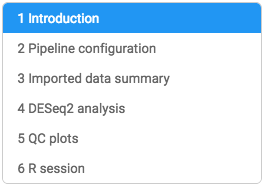
\includegraphics{images/deago_navigation.png}
\caption{Navigation panel}
\end{figure}

    If you click on \textbf{\texttt{Pipeline\ configuration}} you will see
that the report contains the commands used to run the analysis (grey
boxes) and their output. The \textbf{\texttt{Pipeline\ configuration}}
section shows the parameters that were used for the analysis. This can
be useful for finding input/output data, troubleshooting and debugging.

    \begin{figure}[H]
\centering
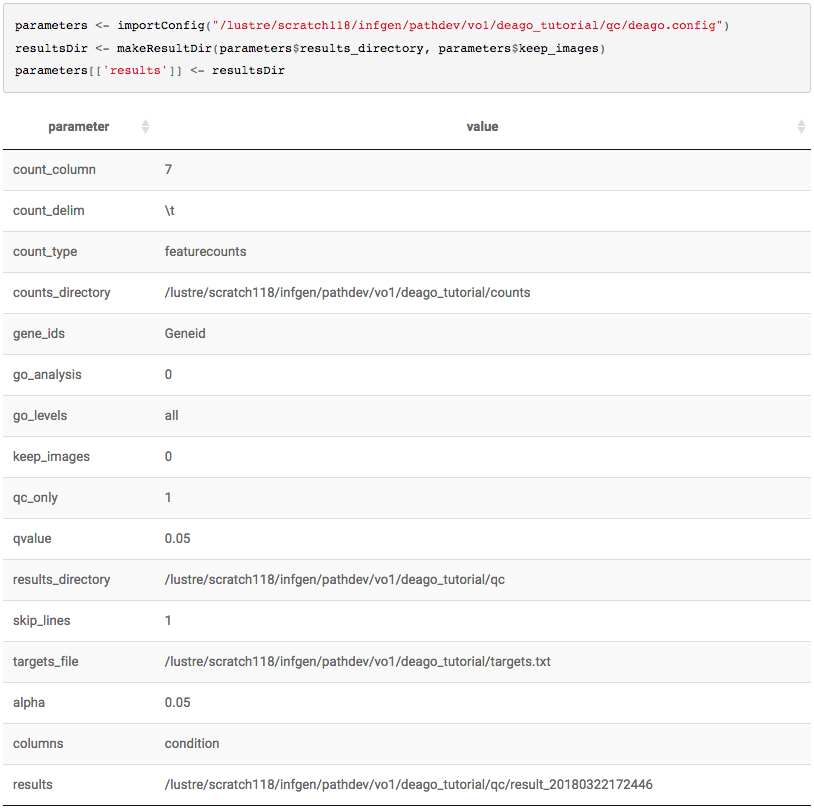
\includegraphics{images/deago_parameters.png}
\caption{Pipeline configuration}
\end{figure}

    To take a look at the QC plots, you can click on
\textbf{\texttt{QC\ Plots}} in the left-hand panel.

First, check to see if there were any problems with the sequencing. The
\textit{Total read counts per sample} plot does what it says on the tin
and shows you the number of reads overlapping features in each sample.
If one sample has a particularly low count compared to the others, it
may indicate an issue and so you should take a closer look at that
sample in some of the other QC plots.

    \begin{figure}[H]
\centering
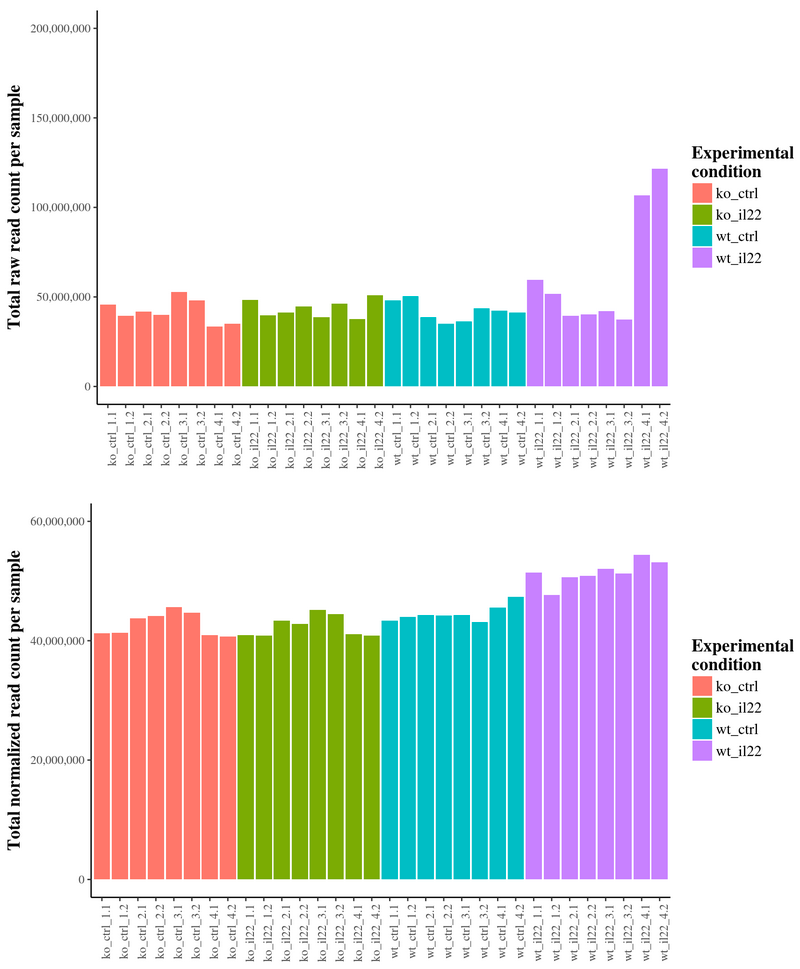
\includegraphics{images/reads_per_sample.png}
\caption{Total read counts per sample plot}
\end{figure}

    The principal component analysis (PCA) and sample-to-sample distances
plot are indicators of variation and will show how well the samples
cluster together. These are a quick way of spotting outliers and
potential batch effects.

In the PCA plot, samples are coloured by condition and the sample labels
are a combination of the sample condition and the replicate number. Here
you will see whether your samples cluster reasonably well with distinct
groups for each condition: \textbf{wt\_ctrl}, \textbf{wt\_il22} and
\textbf{ko\_ctrl}/\textbf{ko\_il22}.

    \begin{figure}[H]
\centering
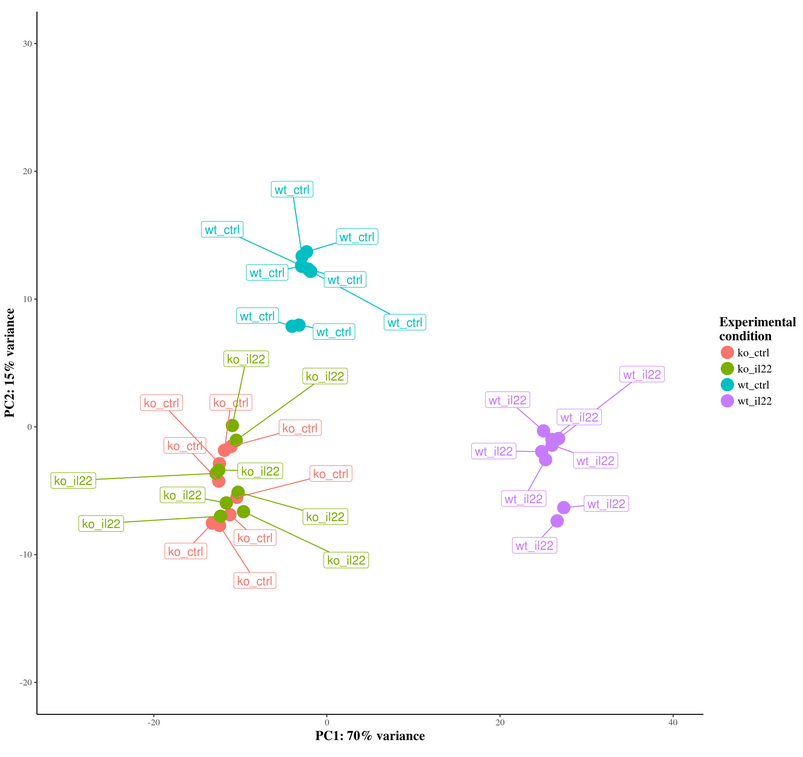
\includegraphics{images/pca.png}
\caption{PCA plot}
\end{figure}

    To compliment the PCA plot, we also have a scree plot which is a
histogram of the percentage contribution of each of the principal
components (PC). The points indicate the cumulative total and the lines
represent broad cutoffs of 70\% and 90\%. Ideally, in a two-factor
analysis we'd hope to see the cumulative total of PC1 and PC2 reaching
70\%, although this may not always be the case.

    \begin{figure}[H]
\centering
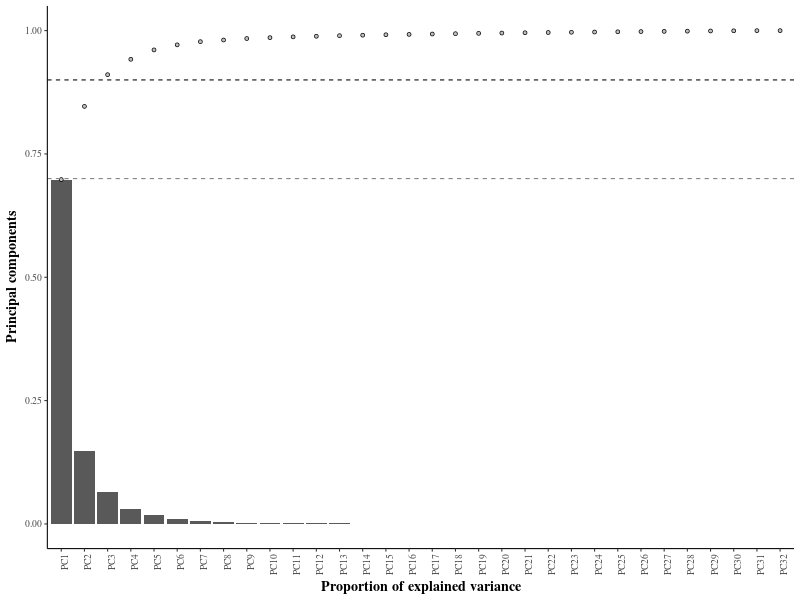
\includegraphics{images/pca_scree.png}
\caption{PCA scree plot}
\end{figure}

    There is also a sample-to-sample distances plot shaded by the distance
(or variability) between samples. The darker the box, the more similar
the samples (or the smaller the distance between them).

    \begin{figure}[H]
\centering
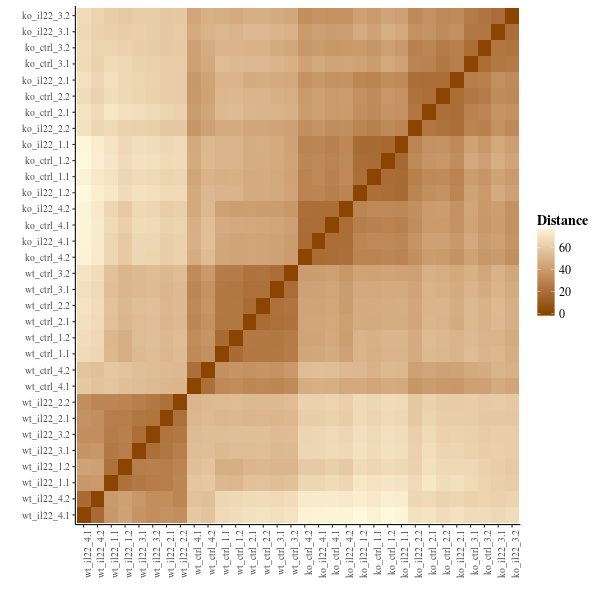
\includegraphics{images/sample_distances.png}
\caption{Sample distances plot}
\end{figure}

    \hypertarget{exercise-3}{%
\subsection{Exercise 3}\label{exercise-3}}

    \textbf{First, let's make sure we're in the \texttt{data} directory.}

\begin{terminalinput}
\begin{Verbatim}[commandchars=\\\{\}]
\llap{\color{black}\LARGE\faKeyboardO\hspace{1em}} \PY{n+nb}{cd} data
\end{Verbatim}
\end{terminalinput}

    \textbf{Each DEAGO analysis should be self-contained, so let's create a
new directory for our QC analysis.}

\begin{terminalinput}
\begin{Verbatim}[commandchars=\\\{\}]
\llap{\color{black}\LARGE\faKeyboardO\hspace{1em}} mkdir qc
\end{Verbatim}
\end{terminalinput}

\begin{terminalinput}
\begin{Verbatim}[commandchars=\\\{\}]
\llap{\color{black}\LARGE\faKeyboardO\hspace{1em}} \PY{n+nb}{cd} qc
\end{Verbatim}
\end{terminalinput}

    \textbf{As this is the first time we're running \texttt{deago} in this
tutorial, let's take a look at the usage.}

\begin{terminalinput}
\begin{Verbatim}[commandchars=\\\{\}]
\llap{\color{black}\LARGE\faKeyboardO\hspace{1em}} deago \PYZhy{}h
\end{Verbatim}
\end{terminalinput}

    Here's a brief explanation of the options we want to use and what they
mean:

\begin{itemize}
\item
  \textbf{\texttt{-\/-build\_config}}~\\
  \textit{tells DEAGO that we want to build a new config file using the
  command line parameters}
\item
  \textbf{\texttt{-c}}~\\
  \textit{tells DEAGO the location of the folder containing our count
  files}
\item
  \textbf{\texttt{-t}}~\\
  \textit{tells DEAGO the location of our sample/condition mapping file}
\item
  \textbf{\texttt{-\/-count\_type}}~\\
  \textit{tells DEAGO the format of the count data (e.g.~featurecounts)
  setting the values for \textbf{count\_column}, \textbf{skip\_lines},
  \textbf{gene\_ids} and \textbf{count\_delim}}
\item
  \textbf{\texttt{-\/-qc}}~\\
  \textit{tells DEAGO to only run the QC analysis}
\end{itemize}

    \textbf{Now, let's get our QC report.}

\begin{terminalinput}
\begin{Verbatim}[commandchars=\\\{\}]
\llap{\color{black}\LARGE\faKeyboardO\hspace{1em}} deago \PYZhy{}\PYZhy{}build\PYZus{}config \PYZhy{}c ../counts \PYZhy{}t ../targets.txt \PY{l+s+se}{\PYZbs{}}
            \PYZhy{}\PYZhy{}count\PYZus{}type featurecounts \PYZhy{}\PYZhy{}qc
\end{Verbatim}
\end{terminalinput}

    \textit{Note: because we are running the analysis from our new \texttt{qc}
directory, we need to us \texttt{../} to say that our directory is one
level above where we are now.}

    \hypertarget{questions}{%
\subsection{Questions}\label{questions}}

\textbf{Q1: Do all the samples have similar total read counts?}

\textbf{Q2: Look at the PCA plot. How many clusters have the samples
grouped into?}

\textbf{Q3: Do you notice anything in the PCA and sample-to-sample
distances plot that you might want to look closer at?}\\
\textit{Hint: look at the groupings in both plots, are there
sub-groupings, do they relate to anything other than the
condition\ldots{}}

\textbf{Q4: What does the \texttt{-\/-keep\_images} option do?}\\
\textit{Hint: look at the DEAGO usage with \texttt{deago\ -h}}

    \hypertarget{whats-next}{%
\subsection{What's next?}\label{whats-next}}

If you want a recap of input file preparation, head back to
\href{input-data.ipynb}{preparing input data}.

Otherwise, let's continue on to
\href{differential-expression.ipynb}{running a differential expression
(DE) analysis}.


    % Add a bibliography block to the postdoc



\newpage






    \hypertarget{running-a-differential-expression-de-analysis}{%
\section{Running a differential expression (DE)
analysis}\label{running-a-differential-expression-de-analysis}}

    \hypertarget{introduction}{%
\subsection{Introduction}\label{introduction}}

By default, DEAGO will run both a quality control (QC) and a
differential expression (DE) analysis. DE analyses try to identify genes
whose expression levels differ between experimental conditions. We don't
normally have enough replicates to do traditional tests of significance
for RNA-Seq data. So, most methods look for outliers in the relationship
between average abundance and fold change and assume most genes are not
differentially expressed.

Rather than just using a fold change threshold to determine which genes
are differentially expressed, DEAs use a variety of statistical tests
for significance. These tests give us a \textbf{p-value} which is an
estimate of how often your observations would occur by chance.

However, we perform these comparisons for each one of the thousands of
genes/transcripts in our dataset. A p-value of 0.01 estimates a
probability of 1\% for seeing our observation just by chance. In an
experiment like ours with 5,000 genes we would expect 5 genes to be
significantly differentially expressed by chance (i.e.~even if there
were no difference between our conditions). Instead of using a p-value
we can use an \textbf{adjusted p-value}, also known as the
\textbf{q-value}, which accounts for the multiple testing and adjusts
the p-value accordingly.

The objectives of this part of the tutorial are:

\begin{itemize}
\tightlist
\item
  run a DE analysis with DEAGO
\item
  interpret the output DE report from DEAGO
\end{itemize}

\hypertarget{input-files}{%
\subsubsection{Input files}\label{input-files}}

We will need to give DEAGO two bits of information:

\begin{itemize}
\item
  \textit{the name/location of the directory containing our gene count
  files (counts)}
\item
  \textit{the name/location of our sample/condition mapping file
  (targets.txt)}
\end{itemize}

We can optionally give DEAGO a formatted annotation file which contains
gene names. These are often more recognisable than the unique gene
identifiers found in the counts files. To do this, we use the
\texttt{-a} option.

\hypertarget{running-a-de-analysis-with-deago}{%
\subsubsection{Running a DE analysis with
DEAGO}\label{running-a-de-analysis-with-deago}}

To run a quick, DE analysis with DEAGO the command would be:

\begin{verbatim}
deago -c <counts_directory> -t <targets file>
\end{verbatim}

As our count files were generated by featureCounts for this tutorial, we
need to also tell DEAGO the count format with the
\texttt{-\/-count\_type} option:

\begin{verbatim}
deago -c <counts_directory> -t <targets file> --count_type featurecounts
\end{verbatim}

As we want to have the gene names in our output tables and plots, we
need to provide our formatted annotation file using the \texttt{-a}
option.

Finally, we will be using the \texttt{-\/-control} option which tells
DEAGO the condition you want to use as your reference or control, in
this case \textbf{WT\_Ctrl}. We use \textbf{\texttt{-\/-control}} to
define our reference condition because, by default, R chooses the
reference condition based on alphabetical order. It would assume that
from our four conditions (\textbf{KO\_Ctrl}, \textbf{KO\_IL22},
\textbf{WT\_Ctrl} and \textbf{WT\_IL22}) that KO\_Ctrl is our reference
condition because it is first alphabetically. The value you use
\textbf{must} be in the condition column in your targets file and is
\textit{case insensitive}.

\begin{verbatim}
deago -c <counts directory> -t <targets file> --count_type featurecounts \
    -a <annotation file> --control <control>
\end{verbatim}

DEAGO also makes an assumption that you want the FDR cutoff (alpha) to
be \textbf{0.05} (default). If you are expecting to use a different
cutoff in your downstream filtering, use the \textbf{\texttt{-q}} option
to define the FDR cutoff (e.g. -q 0.01).

\hypertarget{output-filesdirectories}{%
\subsubsection{Output files/directories}\label{output-filesdirectories}}

Once your DE analysis has finished, you should see several new files and
directories:

\begin{itemize}
\item
  \textbf{\texttt{deago.config}}~\\
  \textit{config file with key/value parameters defining the analysis}
\item
  \textbf{\texttt{deago.rlog}}~\\
  \textit{log of the R output generated when converting the R markdown to
  HTML}
\item
  \textbf{\texttt{deago\_markdown.Rmd}}~\\
  \textit{R markdown used to run the analysis}
\item
  \textbf{\texttt{deago\_markdown.html}}~\\
  \textit{HTML report generated from the R markdown}
\item
  \textbf{\texttt{results\_\textless{}timestammp\textgreater{}}}~\\
  \textit{directory containing unfiltered DE analysis results and
  normalised counts for all genes, one file per contrast}
\end{itemize}

\hypertarget{results-directory}{%
\paragraph{Results directory}\label{results-directory}}

The report tables are limited to genes with an adjusted p-value
\textless{} 0.01 and a log2 fold change \textgreater{}= 2 or
\textless{}= -2. However, you are likely to want to explore and filter
these results using different thresholds. So, DEAGO also writes the
unfiltered results table containing all genes to individual files, one
per contrast in your timestamped results directory.

So, for the full results of the contrast between WT and KO cells treated
with IL22 you would look at:

\begin{verbatim}
results_<timestamp>/wt_il22_vs_ko_il22_q0.05.txt
\end{verbatim}

\hypertarget{de-analysis-report}{%
\subsubsection{DE analysis report}\label{de-analysis-report}}

The output file we're interested in is
\textbf{\texttt{deago\_markdown.html}} which is your DE analysis report.
Go ahead and open it in a web browser (e.g.~Chrome, Firefox, IE,
Safari\ldots{}). You can do this by going to ``File -\textgreater{}
Open'' in the top navigation or (if you have Firefox installed, use the
command:

\begin{terminalinput}
\begin{Verbatim}[commandchars=\\\{\}]
\llap{\color{black}\LARGE\faKeyboardO\hspace{1em}} firefox deago\PYZus{}markdown.html
\end{Verbatim}
\end{terminalinput}

    In addition to the QC sections we saw before, you should now see a new
option in the left-hand sidebar called
\textbf{\texttt{Pairwise\ contrasts}}. Click on it and it will take you
to your DE analysis results.

First there is a \textbf{\texttt{Contrast\ summary}} section which
contains a summary table showing how many genes are up-regulated or
down-regulated in each contrast (comparison between two sample groups).
We can see that there were no differentially expressed (DE) genes
between the knockout (\textbf{KO}) samples induced with IL22
(\textbf{ko\_il22}) and the control knockout samples. However, there
were 860 DE genes between wildtype (\textbf{WT}) and knockout
(\textbf{KO}) samples induced with IL22, 510 up-regulated in the WT
samples compared to the KO samples and 350 down-regulated.

    \begin{figure}[!h]
\centering
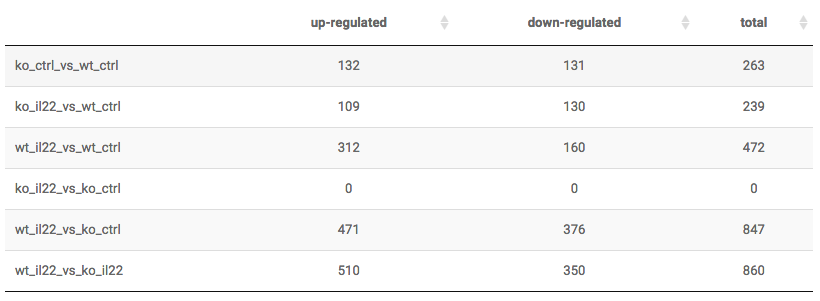
\includegraphics{images/DEsummary.png}
\caption{DE summary table}
\end{figure}

    If there are 2-4 contrasts in the analysis, there will also be a Venn
diagram showing the overlap/differences in total DE genes between
contrasts. We have 6 contrasts in this analysis, so no Venn diagram was
generated, but an example would be:

    \begin{figure}[H]
\centering
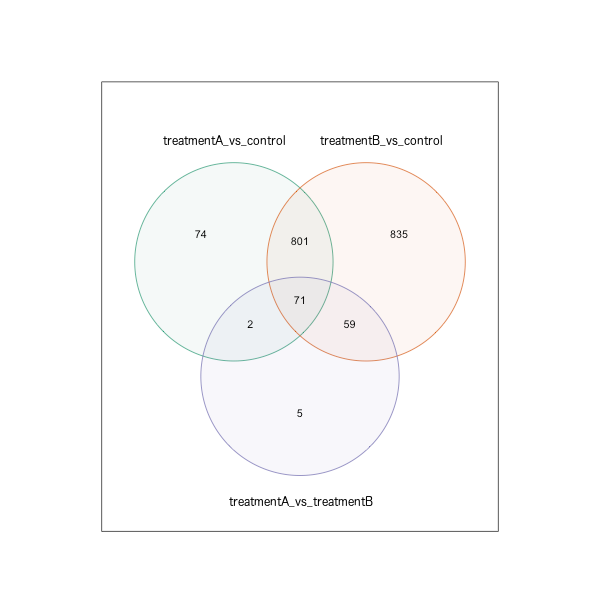
\includegraphics{images/DEvenn.png}
\caption{DE Venn diagram}
\end{figure}

    The DE analysis report then has a series of subsections, one per
contrast. Each contrast section has an MA plot and a volcano plot. The
top 5 up- and down-regulated gene identifiers are labelled on plots. If
an annotation with gene symbols was used then the point labels will be
the gene symbols and not the gene identifiers.

    \begin{figure}[H]
\centering
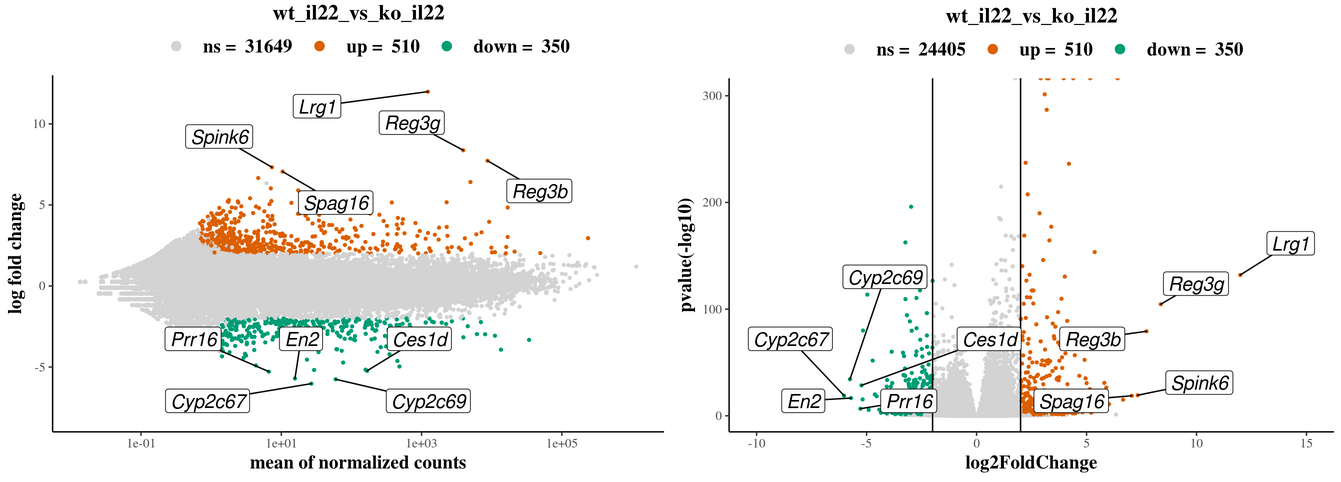
\includegraphics{images/DEvolcanoMA.png}
\caption{DE volcano and MA plots}
\end{figure}

    Each contrast section will also have a DE results table which contains
genes with an adjusted p-value \textless{} 0.01 and a log2 fold change
\textgreater{}= 2 or \textless{}= -2. This is to reduce the number of
genes in the table so that the HTML report is compact and sharable.

    \begin{figure}[H]
\centering
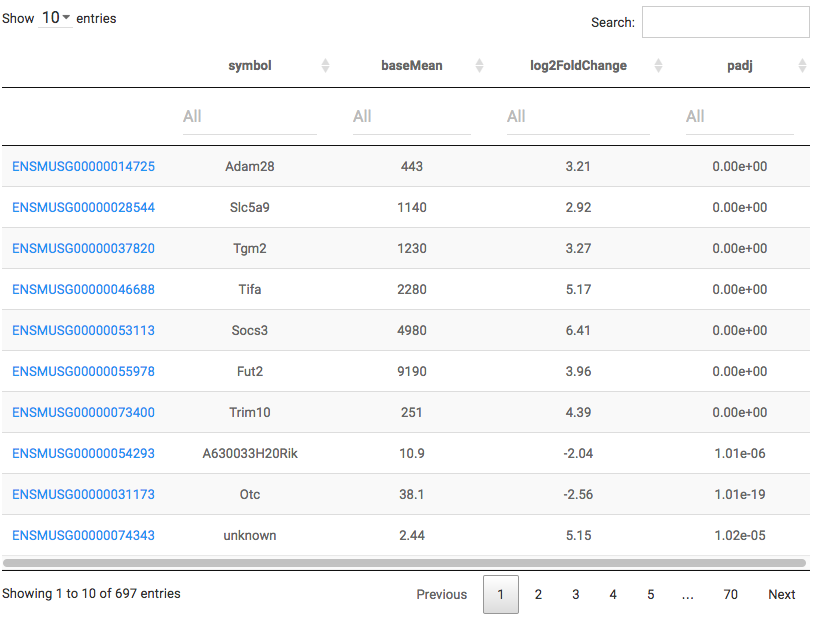
\includegraphics{images/DEtable.png}
\caption{DE contrast results table}
\end{figure}

    These tables contain the DESeq2 results and are where you will find your
adjusted p-values and log2 fold change values. Also, as our gene
identifiers are Ensembl identifiers, they have been converted to a link
and if you click on one, it will take you to the current Ensembl page
for that gene stable ID. In this example, we had include an annotation
in the analysis and so the gene symbols are also shown.

All of the tables are interactive and can be searched or filtered. The
paper describes the up-regulation of \textit{Fut2} by IL-22RA1 signalling,
so let's take a look. The search box at the top right searches the whole
table, so we can use it to search for any \textit{Fut} genes.

    \begin{figure}[H]
\centering
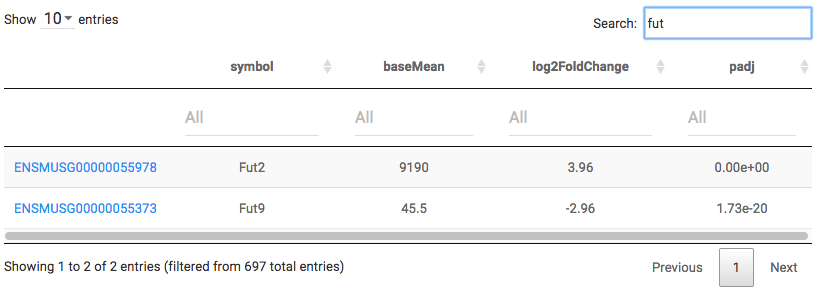
\includegraphics{images/DEsearch.png}
\caption{Searching DE tables}
\end{figure}

    This gives us two genes: \textit{Fut2} and \textit{Fut9}.

Now, say we wanted to only see the up-regulated \textit{Fut} genes. We can
limit searches and filters to a single column by using the search/filter
boxes at the top of each column. Use the selector at the top of the
\textbf{\texttt{log2FoldChange}} column to only include values greater
than 0 (i.e.~drag the left selector).

    \begin{figure}[H]
\centering
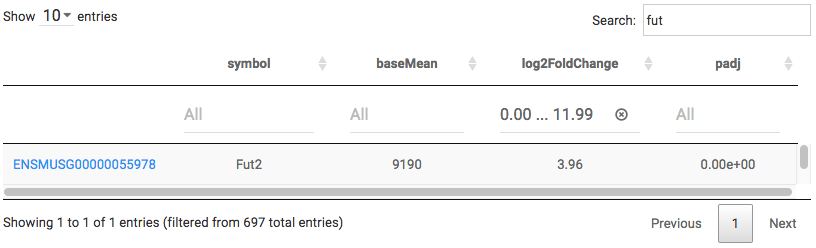
\includegraphics{images/DEfilter.png}
\caption{Searching DE tables}
\end{figure}

    We are now left with the only up-regulated \textit{Fut} gene, \textit{Fut2}.

    \hypertarget{exercise-4}{%
\subsection{Exercise 4}\label{exercise-4}}

\textbf{First, let's make sure we're in the \texttt{data} directory.}

\begin{terminalinput}
\begin{Verbatim}[commandchars=\\\{\}]
\llap{\color{black}\LARGE\faKeyboardO\hspace{1em}}\PY{n+nb}{cd} data
\end{Verbatim}
\end{terminalinput}

    \begin{lstlisting}
(no output)
    \end{lstlisting}

    \textbf{Each DEAGO analysis should be self-contained, so let's create a
new directory for our DE analysis.}

\begin{terminalinput}
\begin{Verbatim}[commandchars=\\\{\}]
\llap{\color{black}\LARGE\faKeyboardO\hspace{1em}} mkdir de\PYZus{}analysis
\end{Verbatim}
\end{terminalinput}

\begin{terminalinput}
\begin{Verbatim}[commandchars=\\\{\}]
\llap{\color{black}\LARGE\faKeyboardO\hspace{1em}}\PY{n+nb}{cd} de\PYZus{}analysis
\end{Verbatim}
\end{terminalinput}

    \begin{lstlisting}
(no output)
    \end{lstlisting}

    \textbf{Now, let's get our DE report.}

\begin{terminalinput}
\begin{Verbatim}[commandchars=\\\{\}]
\llap{\color{black}\LARGE\faKeyboardO\hspace{1em}} deago \PYZhy{}\PYZhy{}build\PYZus{}config \PYZhy{}c ../counts \PYZhy{}t ../targets.txt \PY{l+s+se}{\PYZbs{}}
            \PYZhy{}\PYZhy{}count\PYZus{}type featurecounts \PY{l+s+se}{\PYZbs{}}
            \PYZhy{}a ../ensembl\PYZus{}mm10\PYZus{}deago\PYZus{}formatted.tsv \PY{l+s+se}{\PYZbs{}}
            \PYZhy{}\PYZhy{}control WT\PYZus{}Ctrl
\end{Verbatim}
\end{terminalinput}

    \hypertarget{questions}{%
\subsection{Questions}\label{questions}}

In \href{https://www.ncbi.nlm.nih.gov/pubmed/25263220}{Figure 5C}
(below), the authors have highlighted four genes: \textbf{\textit{Fut2}},
\textbf{\textit{Sec1}}, \textbf{\textit{Fut8}} and \textbf{\textit{B4galt1}}
which are associated with glycosylation.

\begin{figure}[!h]
\centering
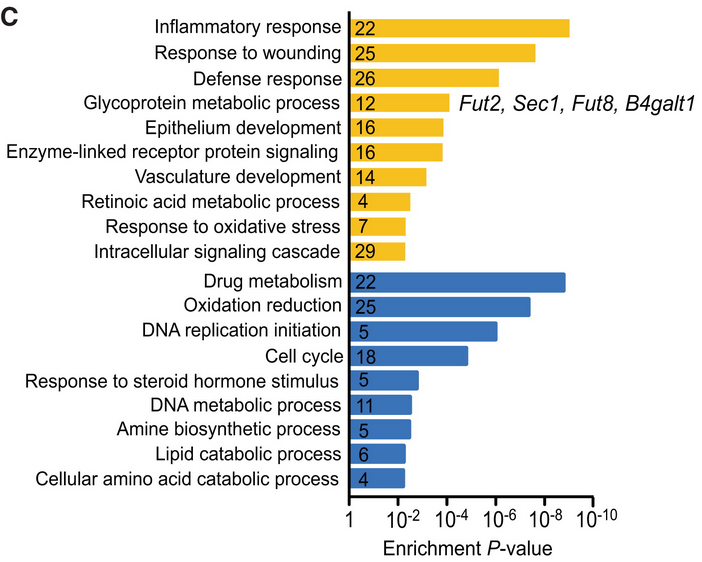
\includegraphics{images/paper_figure5.png}
\caption{GO term enrichment}
\end{figure}

\textbf{We have already found \textit{Fut2}, answer the following
questions for the remaining 3 genes using the contrast results for WT
and KO cells treated with IL22.}

\textbf{Q1: What is the gene identifier (geneID)?}

\textbf{Q2: What is the log2 fold change?}

\textbf{Q3: What is the adjusted p-value?}

\textit{Hint: you may want to use \texttt{awk} to look at columns 36 and
40 in the unfiltered results files for that contrast if the genes are
not found in the report tables}

    \hypertarget{whats-next}{%
\subsection{What's next?}\label{whats-next}}

If you want a recap of input file preparation, head back to
\href{quality-control.ipynb}{running a quality control (QC) analysis}.

Otherwise, let's continue on to \href{go-term-enrichment.ipynb}{running
a GO term enrichment analysis}.


    % Add a bibliography block to the postdoc



\newpage






    \hypertarget{running-a-gene-ontology-go-term-enrichment-analysis}{%
\section{Running a gene ontology (GO) term enrichment
analysis}\label{running-a-gene-ontology-go-term-enrichment-analysis}}

    \hypertarget{introduction}{%
\subsection{Introduction}\label{introduction}}

Once you have your list of differentially expressed (DE) genes, the next
step is often to ask whether the DE genes associated with a particular
biological process or function. To do this, we can perform a gene
ontology (GO) term enrichment analysis. A gene ontology (GO) is a
controlled vocabulary which describes gene products from in any organism
(i.e.~species agnostic). These descriptions are broken down into three
categories:

\begin{itemize}
\item
  \textbf{molecular function (MF)} \textit{what the gene product does}
\item
  \textbf{biological process (BP)} \textit{why the gene product does this}
\item
  \textbf{cell component (CC)} \textit{where the gene product acts}
\end{itemize}

DEAGO uses
\textbf{\href{https://bioconductor.org/packages/release/bioc/html/topGO.html}{topGO}}
to compare a target gene list (e.g.~your DE genes) to the background
(all genes) and identifies GO terms which are significantly enriched or
over-represented in your gene list.

The objectives of this part of the tutorial are:

\begin{itemize}
\tightlist
\item
  run a GO analysis with DEAGO
\item
  interpret the output GO report from DEAGO
\end{itemize}

\hypertarget{input-files}{%
\subsubsection{Input files}\label{input-files}}

We will need to give DEAGO three bits of information:

\begin{itemize}
\item
  \textit{the name/location of the directory containing our gene count
  files (counts)}
\item
  \textit{the name/location of our sample/condition mapping file
  (targets.txt)}
\item
  \textit{the name/location of our formatted annotation file
  (ensembl\_mm10\_deago\_formatted.tsv)}
\end{itemize}

\hypertarget{running-a-go-analysis-with-deago}{%
\subsubsection{Running a GO analysis with
DEAGO}\label{running-a-go-analysis-with-deago}}

To simplest command to run a GO analysis with DEAGO the command would
be:

\begin{verbatim}
deago -c <counts_directory> -t <targets file> -a <annotation file> --go
\end{verbatim}

To indicate that we want to run a GO analysis, we use the
\texttt{-\/-go} option. Notice here that we \textbf{must} provide a
formatted annotation file using the \texttt{-a} option as we need to
know the GO terms assoicated with each gene for the analysis.

However, as before, our count files were generated by featureCounts for
this tutorial, so we need to also tell DEAGO the count format with the
\texttt{-\/-count\_type} option:

\begin{verbatim}
deago -c <counts_directory> -t <targets file> -a <annotation file> --go \
    --count_type featurecounts
\end{verbatim}

We're also using the \texttt{-\/-control} option, as before, which tells
DEAGO the condition you want to use as your reference or control, in
this case \textbf{WT\_Ctrl}.

\begin{verbatim}
deago -c <counts_directory> -t <targets file> -a <annotation file> --go\
    --count_type featurecounts --control <control>
\end{verbatim}

\hypertarget{output-files}{%
\subsubsection{Output files}\label{output-files}}

Once your GO analysis has finished, you should see several new files and
directories:

\begin{itemize}
\item
  \textbf{\texttt{deago.config}}~\\
  \textit{config file with key/value parameters defining the analysis}
\item
  \textbf{\texttt{deago.rlog}}~\\
  \textit{log of the R output generated when converting the R markdown to
  HTML}
\item
  \textbf{\texttt{deago\_markdown.Rmd}}~\\
  \textit{R markdown used to run the analysis}
\item
  \textbf{\texttt{deago\_markdown.html}}~\\
  \textit{HTML report generated from the R markdown}
\item
  \textbf{\texttt{results\_\textless{}timestammp\textgreater{}}}~\\
  \textit{directory containing unfiltered DE analysis results and
  normalised counts for all genes, one file per contrast}
\end{itemize}

\hypertarget{results-directory}{%
\paragraph{Results directory}\label{results-directory}}

DEAGO also writes the GO term enrichment analysis results tables
containing the top 30 significantly enriched GO terms to individual
files, split by GO term level (MF and BP), in your timestamped results
directory. If possible, there will be three GO tables for each GO term
level containing the results for analyses using all genes, up-regulated
genes only and down-regulated genes

\begin{itemize}
\tightlist
\item
  {[}contrast{]}\_BP.tsv
\item
  {[}contrast{]}\_BP\_up.tsv
\item
  {[}contrast{]}\_BP\_down.tsv
\item
  {[}contrast{]}\_MF.tsv
\item
  {[}contrast{]}\_MF\_up.tsv
\item
  {[}contrast{]}\_MF\_down.tsv
\end{itemize}

\hypertarget{go-analysis-report}{%
\subsubsection{GO analysis report}\label{go-analysis-report}}

The output file we're interested in is deago\_markdown.html which is
your GO analysis report. Go ahead and open it in a web browser
(e.g.~Chrome, Firefox, IE, Safari\ldots{}). You can do this by going to
``File -\textgreater{} Open'' in the top navigation or (if you have
Firefox installed, use the command:

\begin{terminalinput}
\begin{Verbatim}[commandchars=\\\{\}]
\llap{\color{black}\LARGE\faKeyboardO\hspace{1em}} firefox deago\PYZus{}markdown.html
\end{Verbatim}
\end{terminalinput}

    You'll already be familiar with the \textbf{\texttt{QC\ plots}} and
\textbf{\texttt{Pairwise\ contrasts}} sections. Click on
\textbf{\texttt{Pairwise\ contrasts}} and then go to the contrast
subsection for \textbf{\texttt{wt\_il22\_vs\_ko\_il22}}. You should now
see six new subsections, \textit{6.7.2 - 6.7.7}, which contain your GO
term enrichment analysis results for that contrast.

The first three subsections have the prefix
\textbf{\texttt{GO\ term\ enrichment\ -\ BP}} and contain the results
for the \textit{Biological Processes (BP)}. The remaining three
subsections have the prefix
\textbf{\texttt{GO\ term\ enrichment\ -\ MF}} and contain the results
for the \textit{Molecular Functions (MF)}.

For each GO level (BP or MF) there is a subsection containing the
results from GO term enrichment analyses which were run using all DE
genes, up-regulated genes only and down-regulated genes only.

Let's take a look at the BP (upregulated genes only) table for the
contrast wt\_il22\_vs\_ko\_il22 (subsection 6.7.3). All of the results
tables are interactive. Despite performing a single-factor analyis, we
can still find the top GO description for up-regulated genes
\textit{inflammatory response} in our results table (GO:0006954).

    \begin{figure}[!h]
\centering
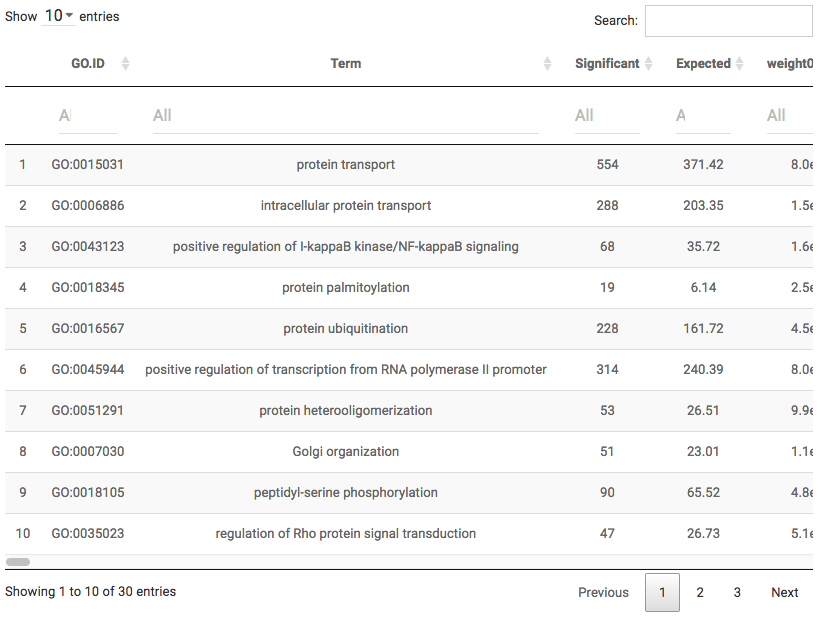
\includegraphics{images/BPupTable.png}
\caption{GO term enrichment results table for wt\_il22\_vs\_ko\_il22 BP
(upregulated genes only)}
\end{figure}

    The paper also mentions \textit{Prdm1} which is upregulated by IL-22RA1
signalling and is a susceptibility gene in to inflammatory bowel
disease. Let's see whether it's associated with any of the enriched GO
terms. Type ``prdm1'' in the top right search box to search the whole
table.

    \begin{figure}[H]
\centering
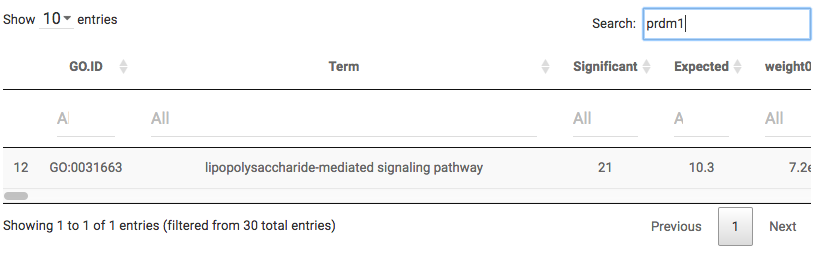
\includegraphics{images/BPupPrdm1Left.png}
\caption{Search for Prdm1 (left)}
\end{figure}

    We can see that one GO term matches: GO:0031663
(lipopolysaccharide-mediated signaling pathway).

Scrolling to the right, we can see how the search found this match. For
each GO term, the DE genes which are associated with that term are also
shown in the table.

    \begin{figure}[H]
\centering
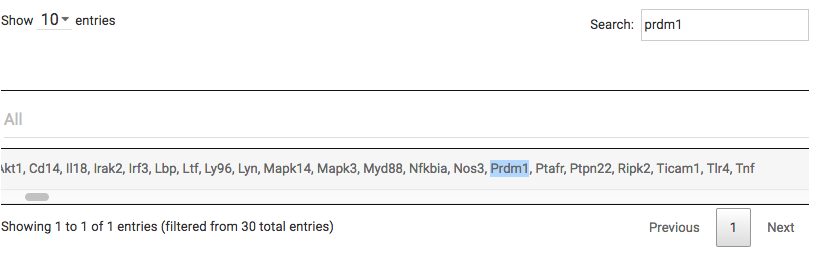
\includegraphics{images/BPupPrdm1Right.png}
\caption{Search for Prdm1 (right)}
\end{figure}

    \hypertarget{exercise-5}{%
\subsection{Exercise 5}\label{exercise-5}}

\textbf{First, let's make sure we're in the data directory.}

\begin{terminalinput}
\begin{Verbatim}[commandchars=\\\{\}]
\llap{\color{black}\LARGE\faKeyboardO\hspace{1em}} \PY{n+nb}{cd} data
\end{Verbatim}
\end{terminalinput}

    \textbf{Each DEAGO analysis should be self-contained, so let's create a
new directory for our GO analysis.}

\begin{terminalinput}
\begin{Verbatim}[commandchars=\\\{\}]
\llap{\color{black}\LARGE\faKeyboardO\hspace{1em}} mkdir go\PYZus{}analysis
\end{Verbatim}
\end{terminalinput}

\begin{terminalinput}
\begin{Verbatim}[commandchars=\\\{\}]
\llap{\color{black}\LARGE\faKeyboardO\hspace{1em}} \PY{n+nb}{cd} go\PYZus{}analysis
\end{Verbatim}
\end{terminalinput}

    \textbf{Now, let's get our GO report.}

\begin{terminalinput}
\begin{Verbatim}[commandchars=\\\{\}]
\llap{\color{black}\LARGE\faKeyboardO\hspace{1em}} deago \PYZhy{}\PYZhy{}build\PYZus{}config \PYZhy{}c ../counts \PYZhy{}t ../targets.txt \PY{l+s+se}{\PYZbs{}}
            \PYZhy{}\PYZhy{}count\PYZus{}type featurecounts \PY{l+s+se}{\PYZbs{}}
            \PYZhy{}a ../ensembl\PYZus{}mm10\PYZus{}deago\PYZus{}formatted.tsv \PY{l+s+se}{\PYZbs{}}
            \PYZhy{}\PYZhy{}control WT\PYZus{}Ctrl \PYZhy{}go
\end{Verbatim}
\end{terminalinput}

    \hypertarget{questions}{%
\subsection{Questions}\label{questions}}

In \href{https://www.ncbi.nlm.nih.gov/pubmed/25263220}{Figure 5C}
(below), the authors have highlighted four genes: \textbf{\textit{Fut2}},
\textbf{\textit{Sec1}}, \textbf{\textit{Fut8}} and \textbf{\textit{B4galt1}}
which are associated with glycosylation.

\begin{figure}[H]
\centering
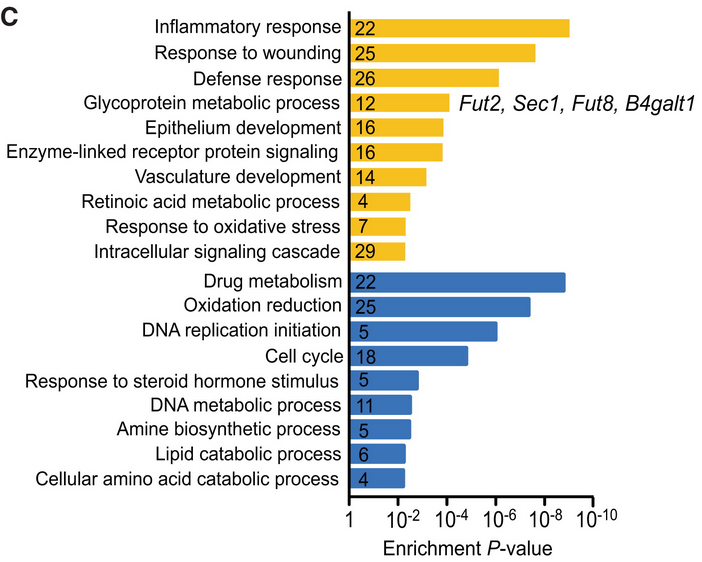
\includegraphics{images/paper_figure5.png}
\caption{GO term enrichment}
\end{figure}

\textbf{Answer the following question for all four genes:}

\textbf{Q1: Which biological processes is this upregulated gene
associated with?}

    \hypertarget{whats-next}{%
\subsection{What's next?}\label{whats-next}}

If you want a recap of input file preparation, head back to
\href{differential-expression.ipynb}{running a differential expression
(DE) analysis}.

Otherwise, let's continue on to
\href{troubleshooting.ipynb}{troubleshooting}.


    % Add a bibliography block to the postdoc



\newpage






    \hypertarget{troubleshooting}{%
\section{Troubleshooting}\label{troubleshooting}}

    If \textbf{\texttt{deago\_markdown.html}} isn't generated, the first
thing to do is check the end of the R log file
(\textbf{\texttt{deago.rlog}}). If successful it should be similar to:

\begin{verbatim}
output file: deago_markdown.knit.md

/software/pathogen/external/apps/usr/bin/pandoc +RTS -K512m -RTS deago_markdown.utf8.md --to html --from
markdown+autolink_bare_uris+ascii_identifiers+tex_math_single_backslash --output /lustre/scratch118/infgen/pathdev
/vo1/deago_tutorial_test/deago_analysis/deago_markdown.html --smart --email-obfuscation none --self-contained
--standalone --section-divs --table-of-contents --toc-depth 3 --variable toc_float=1 --variable
toc_selectors=h1,h2,h3 --variable toc_collapsed=1 --variable toc_smooth_scroll=1 --variable toc_print=1
--template /software/pathogen /external/lib/R-3.4/rmarkdown/rmd/h/default.html --no-highlight
--variable highlightjs=1 --number-sections --variable 'theme:paper' --include-in-header
/tmp/RtmpyTxHuS/rmarkdown-str1782209e9bc2.html --mathjax --variable
'mathjax-url:https://mathjax.rstudio.com/latest/MathJax.js?config=TeX-AMS-MML_HTMLorMML'

In addition: Warning messages:
1: Removed 778 rows containing non-finite values (stat_density).
2: Removed 778 rows containing non-finite values (stat_density).
\end{verbatim}

If not, it will show the error which stopped the report being generated.
For example:

Quitting from lines 206-208 (deago\_markdown.Rmd)

\begin{verbatim}
Error in .local(.Object, ...) : allGenes must be a factor with 2 levels
Calls: <Anonymous> ... prepareGOdata -> new -> initialize -> initialize -> .local
In addition: Warning messages:
1: Removed 778 rows containing non-finite values (stat_density).
2: Removed 778 rows containing non-finite values (stat_density).

Execution halted
\end{verbatim}

This suggests you should look at what's on lines 206-208 in
\textbf{\texttt{deago\_markdown.Rmd}} and try to work out the cause of
the error. Once you've fixed it, you can use
\textbf{\texttt{deago\_markdown\_to\_html}} to try and convert your
modified markdown file to a new HTML report. If this doesn't work, you
can always try running the commands from the markdown file in R manually
to debug the issue.

If this doesn't work and you think there might be bug, please email
\href{mailto:path-help@sanger.ac.uk}{\nolinkurl{path-help@sanger.ac.uk}}
attaching your R markdown file, R log file and config file.

    \textbf{Congratulations, you have now reached the end of this tutorial!}

To go back to the beginning, you'll want to head to the
\href{index.ipynb}{introduction}. Or, for the answers to the tutorial
questions, head to the answer section (answers.ipynb).


    % Add a bibliography block to the postdoc



\end{document}
